\documentclass[letterpaper]{article}

\usepackage{amsmath}
\usepackage{gensymb}
\usepackage[vmargin=1in,hmargin=1.25in]{geometry}
\usepackage{graphicx}
\usepackage{hyperref}
\usepackage{microtype}
\usepackage{lmodern}

\title{ECE/CSE 576, Spring 2019 Homework 3: Content-Based Image Retrieval}
\author{Philip Pham}
\date{\today}

\begin{document}
\maketitle

\section{Algorithm}

For each image, we performed $k$-means clustering with $k = 8$ for 32
iterations.\footnote{A random seed of 2020 was used for reproducibility.}
Connected components was then applied to segment the image into contiguous
regions. Only regions that made up at least $1/256$ of the image were kept.

For each region, the following features were computed: (1) the proportion of the
image occupied the region, (2) the average red, green, and blue color levels
scaled to lie in range $[0,1]$, (3) the centroid, (4) the bounding box, and (5)
a normalized gray-level co-occurrence matrix (GLCM).

For the centroid and bounding box, coordinates were scaled to lie in range
$[0, 1]$. The gray-levels were binned into 8 buckets each of size 32. The
neighboring pixel of $(r, c)$ was the diagonal pixel at
$\left(r^\prime = r + 1, c^\prime = c + 1\right)$. The GLCM was initialized with
entries of $0.1$ which corresponds to putting a Dirichlet prior on
$\operatorname{GrayLevel}\left(r^\prime, c^\prime\right) \mid
\operatorname{GrayLevel}\left(r, c\right)$ with $\alpha = 0.1$. After counting
co-occurrences, the matrix was normalized to define a proper joint probability
distribution over the gray levels of a pixel and its neighbor.

\subsection{Distance 1}

Let $\mathbf{q}$ be the query feature vector and $\mathbf{p}$ be feature vector
for another image in the database. Distance 1 was simply the squared Euclidean
distance over the 5 classes of features:
\begin{equation}
  d_1\left(\mathbf{q}, \mathbf{p}\right) = \left\lVert \mathbf{q} - \mathbf{p}\right\rVert_2^2.
  \label{eqn:distance_1}
\end{equation}
For the vectors in Equation \ref{eqn:distance_1}, the first coordinate is the
volume, the colors are the next 3 entries, the centroid are the next 2 entries
in the vector, the top, right, bottom, and left of the bounding box make the
next 4 entries, and the normalized GLCM are the last 64 entries for a total of
$p = 74$ features per a feature vector.

\subsection{Distance 2}

The second distance function is more complex and uses several derived features.
\begin{equation}
  d_2\left(\mathbf{q}, \mathbf{p}\right) = V(\mathbf{q})\left[\left(V(\mathbf{q}) - V(\mathbf{p})\right)^2 +
  d_{2,\text{Color}}\left(\mathbf{p}, \mathbf{q}\right) +
  d_{2,\text{Position}}\left(\mathbf{p}, \mathbf{q}\right) +
  d_{2,\text{GLCM}}\left(\mathbf{p}, \mathbf{q}\right)\right],
  \label{eqn:distance_2}
\end{equation}
where $V: \mathcal{R} \rightarrow [0, 1]$ is a function mapping a region into
the percentage of the image occupied. Suppose the query vector has region
vectors $\left\{\mathbf{q}_i\right\}_{i=1}^{N}$ and another image has region
vectors $\left\{\mathbf{p}_j\right\}_{j=1}^{M}$. The total distance to the image
given a metric $d$ is computed as
\begin{equation}
  D_d\left(\left\{\mathbf{q}_i\right\}_{i=1}^{N}, \left\{\mathbf{p}_j\right\}_{j=1}^{M}\right)
  = \frac{1}{N}\sum_{i=1}^N\min_{j}\left\{d\left(\mathbf{q}_i, \mathbf{p}_j\right)\right\},
  \label{eqn:total_distance}
\end{equation}
so the leading $V\left(\mathbf{q}\right)$ factor in Equation
\ref{eqn:distance_2} assigns more importance to larger regions.

Let $\operatorname{rgb}: \mathcal{R}\rightarrow \left[0, 1\right]^3$ map a
region to the average color levels. Then, we define
\begin{equation}
  \begin{split}
  d_{2,\text{Color}}\left(\mathbf{q}, \mathbf{p}\right) =
  \left(\left\lVert \operatorname{rgb}\left(\mathbf{q}\right)\right\rVert_2 -
    \left\lVert \operatorname{rgb}\left(\mathbf{p}\right)\right\rVert_2\right)^2
  &+ \left\lVert \operatorname{rgb}\left(\mathbf{q}\right) -
    \operatorname{rgb}\left(\mathbf{p}\right)
  \right\rVert_1 \\ &+
  \left(1 - \frac{\operatorname{rgb}\left(\mathbf{q}\right)\cdot\operatorname{rgb}\left(\mathbf{p}\right)}
    {\left\lVert \operatorname{rgb}\left(\mathbf{q}\right)\right\rVert_2\left\lVert \operatorname{rgb}\left(\mathbf{p}\right)\right\rVert_2}\right),
\end{split}
  \label{eqn:distance_2_color}  
\end{equation}
where the first term penalizes differing magnitude, the second term is the $l_1$
distance, and the third term is the cosine distance.

Let $\operatorname{Row}: \mathcal{R} \rightarrow \left[0, 1\right]$ and
$\operatorname{Col}: \mathcal{R} \rightarrow \left[0, 1\right]$ be the relative
row and columns for a region. Given two region bounding boxes, we can compute
the \href{https://en.wikipedia.org/wiki/Jaccard_index}{Jaccard index} also know
as \emph{intersection over union}. Denote the map
$J: \mathcal{R} \times \mathcal{R} \rightarrow [0,1]$. Based on the centroid and
bounding box, we define
\begin{equation}
  \begin{split}
  d_{2,\text{Position}}\left(\mathbf{q}, \mathbf{p}\right)
  = \frac{1}{2}\left(
    \operatorname{Row}\left(\mathbf{q}\right) - \operatorname{Row}\left(\mathbf{p}\right)
    \right)^2 &+
    \frac{1}{2}\left(
      \operatorname{Col}\left(\mathbf{q}\right) - \operatorname{Col}\left(\mathbf{p}\right)
    \right)^2 \\
    &+ \left(1 - J\left(\mathbf{p}, \mathbf{q}\right)\right)^2.
  \end{split}
  \label{eqn:distance_2_position}
\end{equation}
The first two terms penalize regions located in the different areas by their
centroids. The last term uses the region bounding boxes and penalizes regions
without a lot of overlap, whether because they are located in different parts of
the images or their sizes differ considerably.

From the normalized $8 \times 8$ GLCM, $N_{\text{GLCM}}\left(\mathbf{q}\right)$,
the auxiliary features \emph{Contrast}, \emph{Energy}, and \emph{Entropy} can
be defined:
\begin{align}
  \operatorname{Contrast}\left(
  \mathbf{q}
  \right) &= \sum_{i=1}^8\sum_{j=1}^8\left(i - j\right)^2
            N_{\text{GLCM}}\left(\mathbf{q}\right)(i, j) \\
  \operatorname{Energy}\left(
  \mathbf{q}
  \right) &= \sum_{i=1}^8\sum_{j=1}^8
            \left[N_{\text{GLCM}}\left(\mathbf{q}\right)(i, j)\right]^2 \\
  \operatorname{Entropy}\left(
  \mathbf{q}
  \right) &= -\sum_{i=1}^8\sum_{j=1}^8
            N_{\text{GLCM}}\left(\mathbf{q}\right)(i, j)\log_2N_{\text{GLCM}}\left(\mathbf{q}\right)(i, j).
\end{align}

Because of differing scales and levels of importance, we defined
\begin{equation}
  \begin{split}
  d_{2,\text{GLCM}}\left(\mathbf{q}, \mathbf{p}\right)
  &= 2\left[
    \operatorname{Contrast}\left(\mathbf{q}\right) -
    \operatorname{Contrast}\left(\mathbf{p}\right)
  \right]^2 \\
  &+ \frac{1}{2}\left[
    \operatorname{Energy}\left(\mathbf{q}\right) -
    \operatorname{Energy}\left(\mathbf{p}\right)
  \right]^2 \\
  &+ \frac{1}{2}\left[
    \operatorname{Entropy}\left(\mathbf{q}\right) -
    \operatorname{Entropy}\left(\mathbf{p}\right)
  \right]^2.
  \end{split}
  \label{eqn:distance_2_glcm}
\end{equation}
as a weighted sum of square differences.

\section{Discussion}

Both distances have the property that if $\mathbf{p} = \mathbf{q}$,
$d\left(\mathbf{p}, \mathbf{q}\right) = 0$, so if the image is in the
database, the image itself will always be returned as the top result.

Color features were found to be very important which explains why a simple
metric like $d_1$ can often be successful. In more complex images, weighting by
the region size, taking into account position with the bounding box, and using
contrast for texture analysis improved retrieval significantly. $d_2$ almost
always outperformed $d_1$ by taking into account these features.

Results of empirical validation are shown in the next section.

\section{Empirical Results}

\subsection{\texttt{beach}}
\begin{center}
  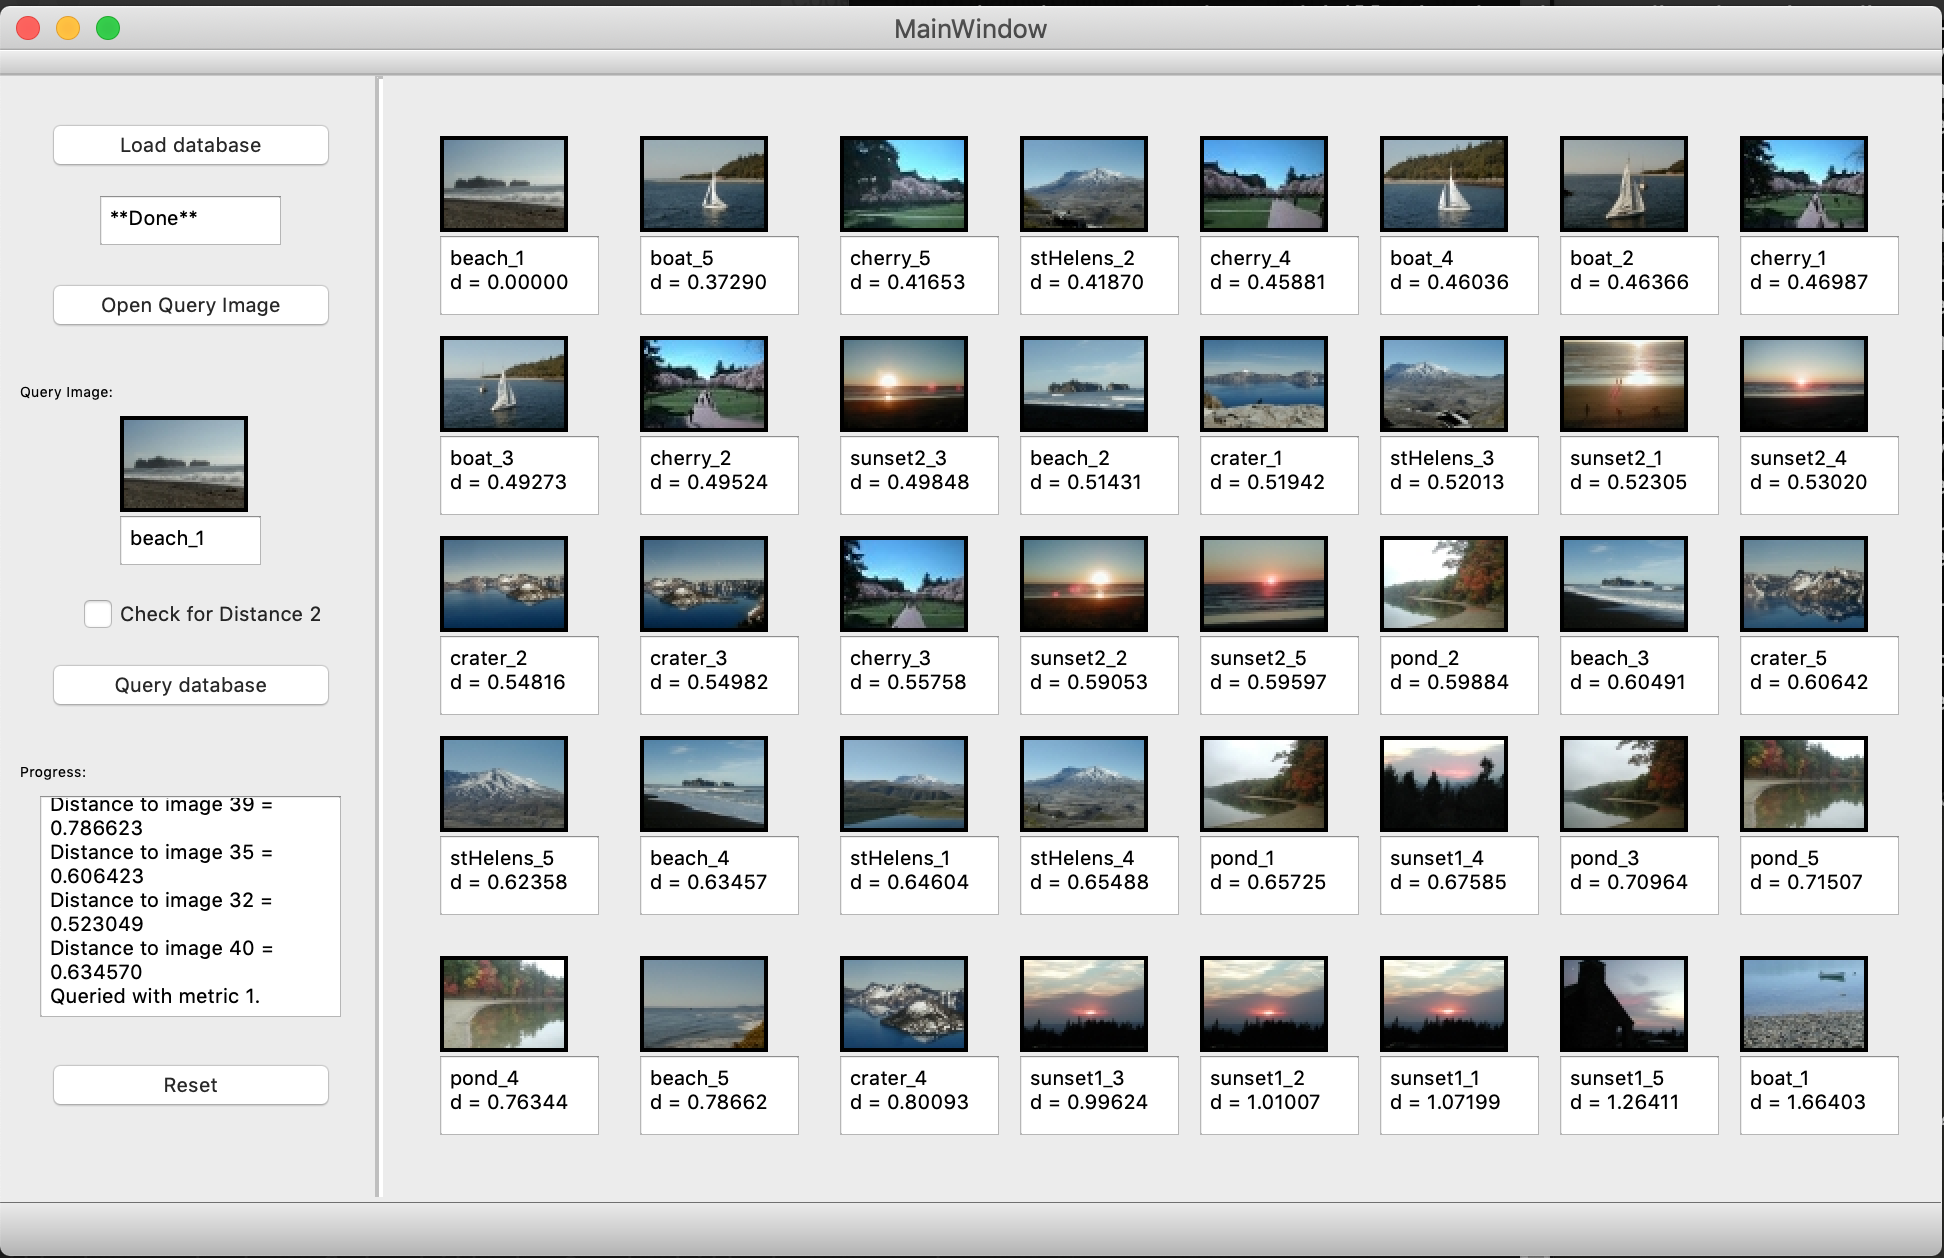
\includegraphics[width=\textwidth]{beach_1_distance1.png}
  
  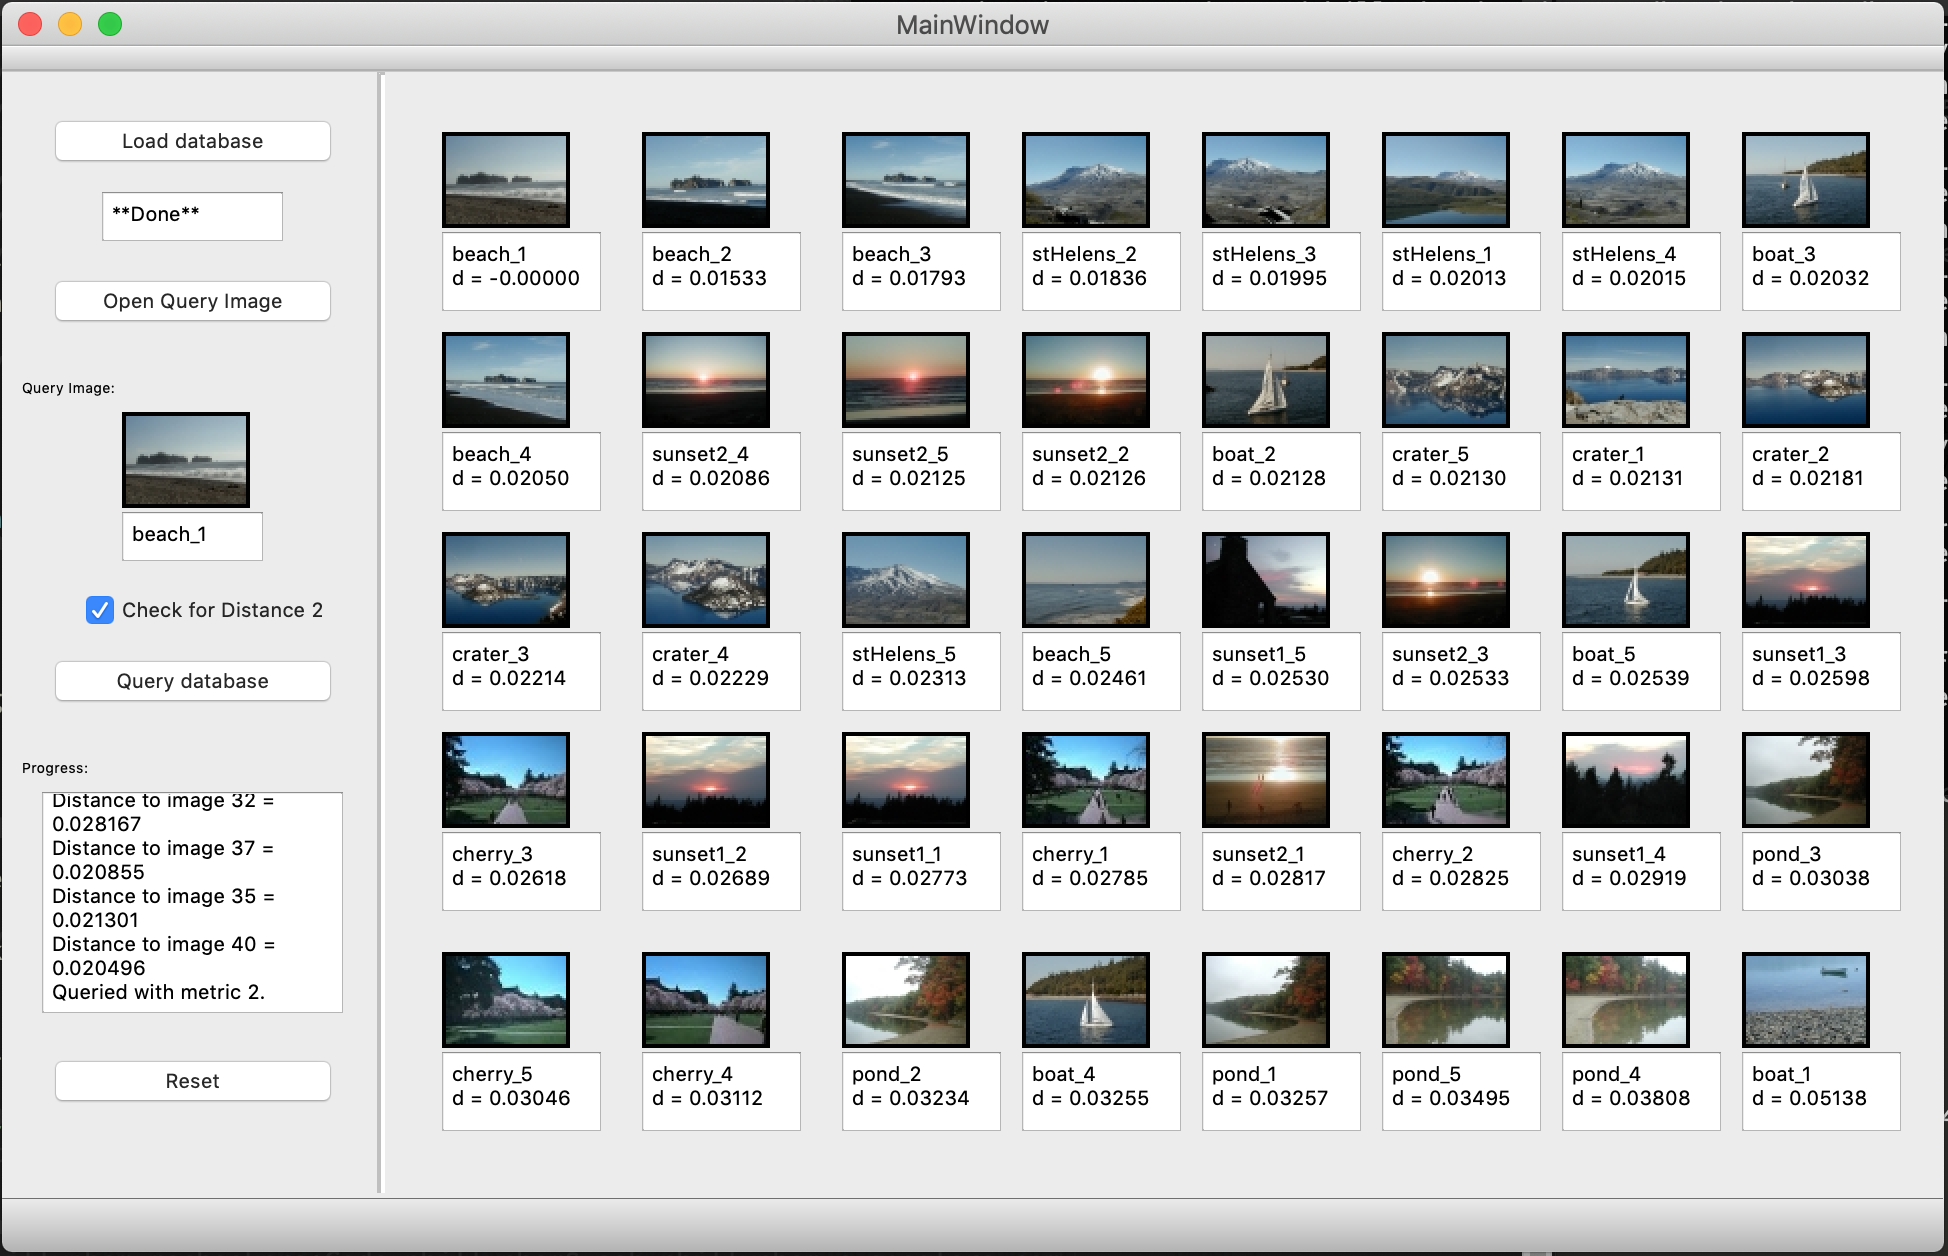
\includegraphics[width=\textwidth]{beach_1_distance2.png}
  
  Query results for \texttt{beach\_1.jpg}.
\end{center}

The beach queries proved challenging. Euclidean distance completely fails, while
$d_2$ only manages to return $2/4$ beach images. Returning an additional beach
image in the top row, $d_2$ does better.

\subsection{\texttt{boat}}
\begin{center}
  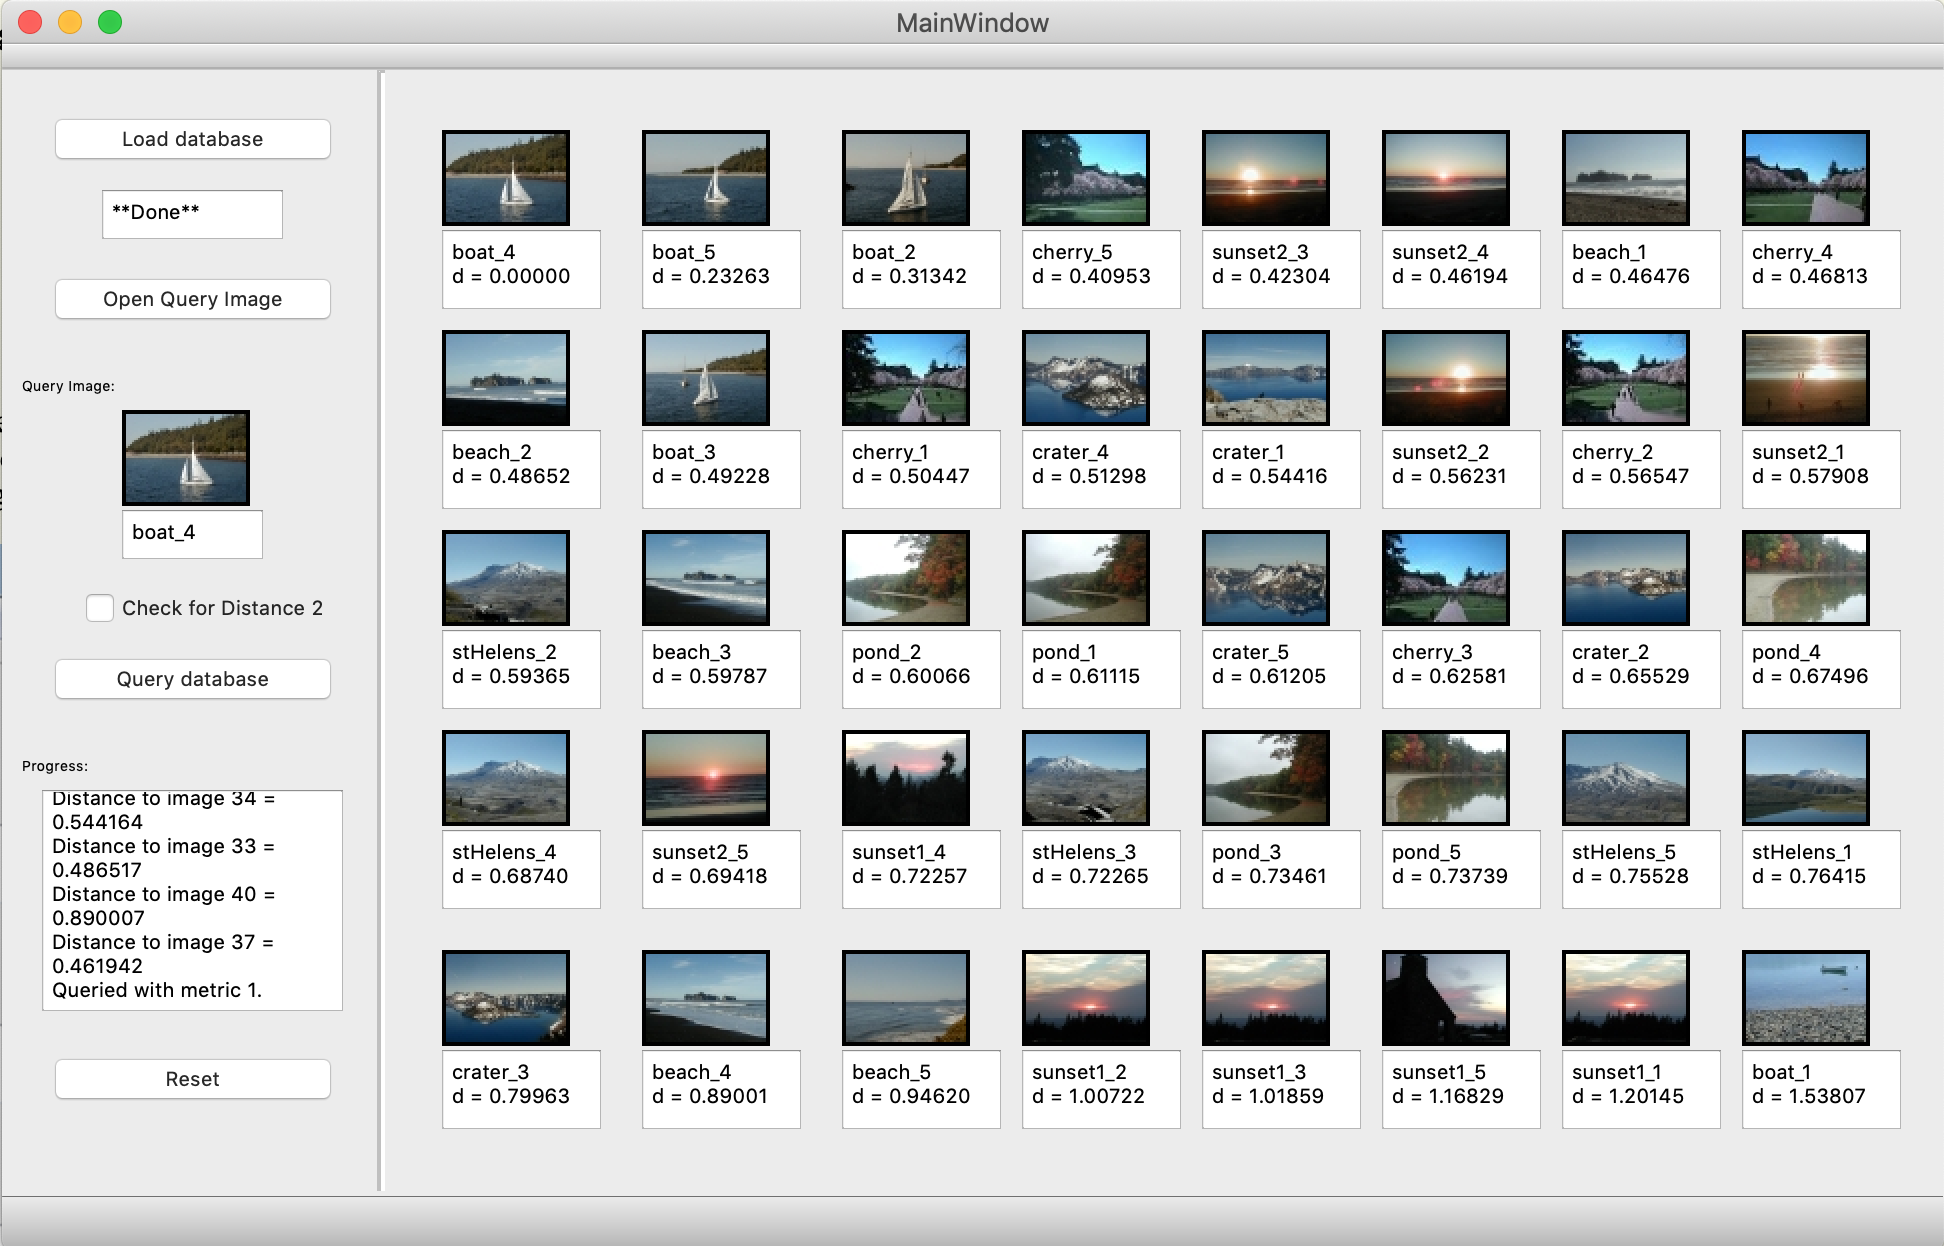
\includegraphics[width=\textwidth]{boat_4_distance1.png}
  
  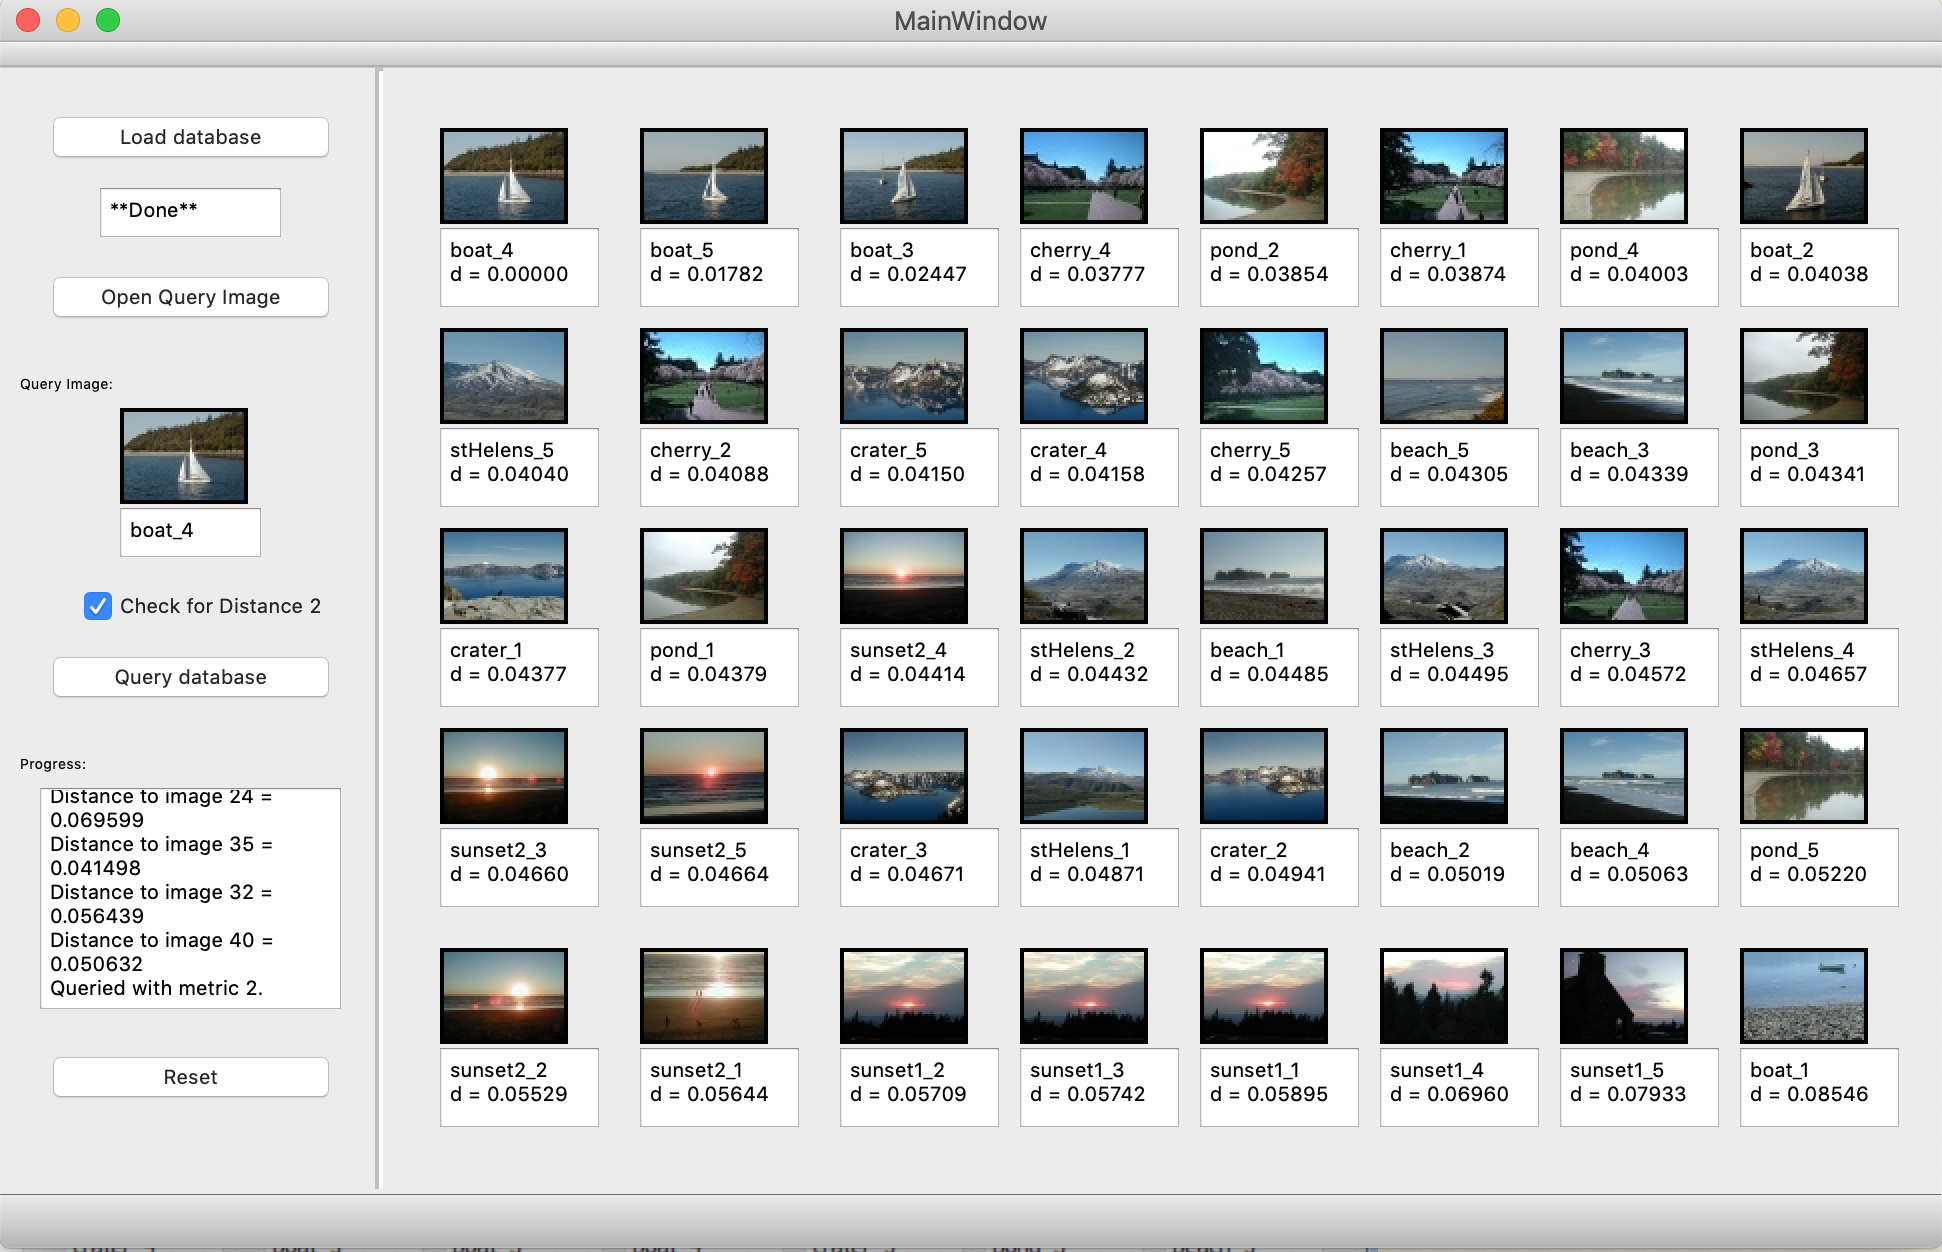
\includegraphics[width=\textwidth]{boat_4_distance2.png}
  
  Query results for \texttt{boat\_4.jpg}.
\end{center}

$d_1$ and $d_2$ both return other boat images for their top two results. One
might say that $d_2$ does slightly better since it has another boat result in
the top row. The boat in \texttt{boat\_1} is too different and not matched.

\subsection{\texttt{cherry}}

\begin{center}
  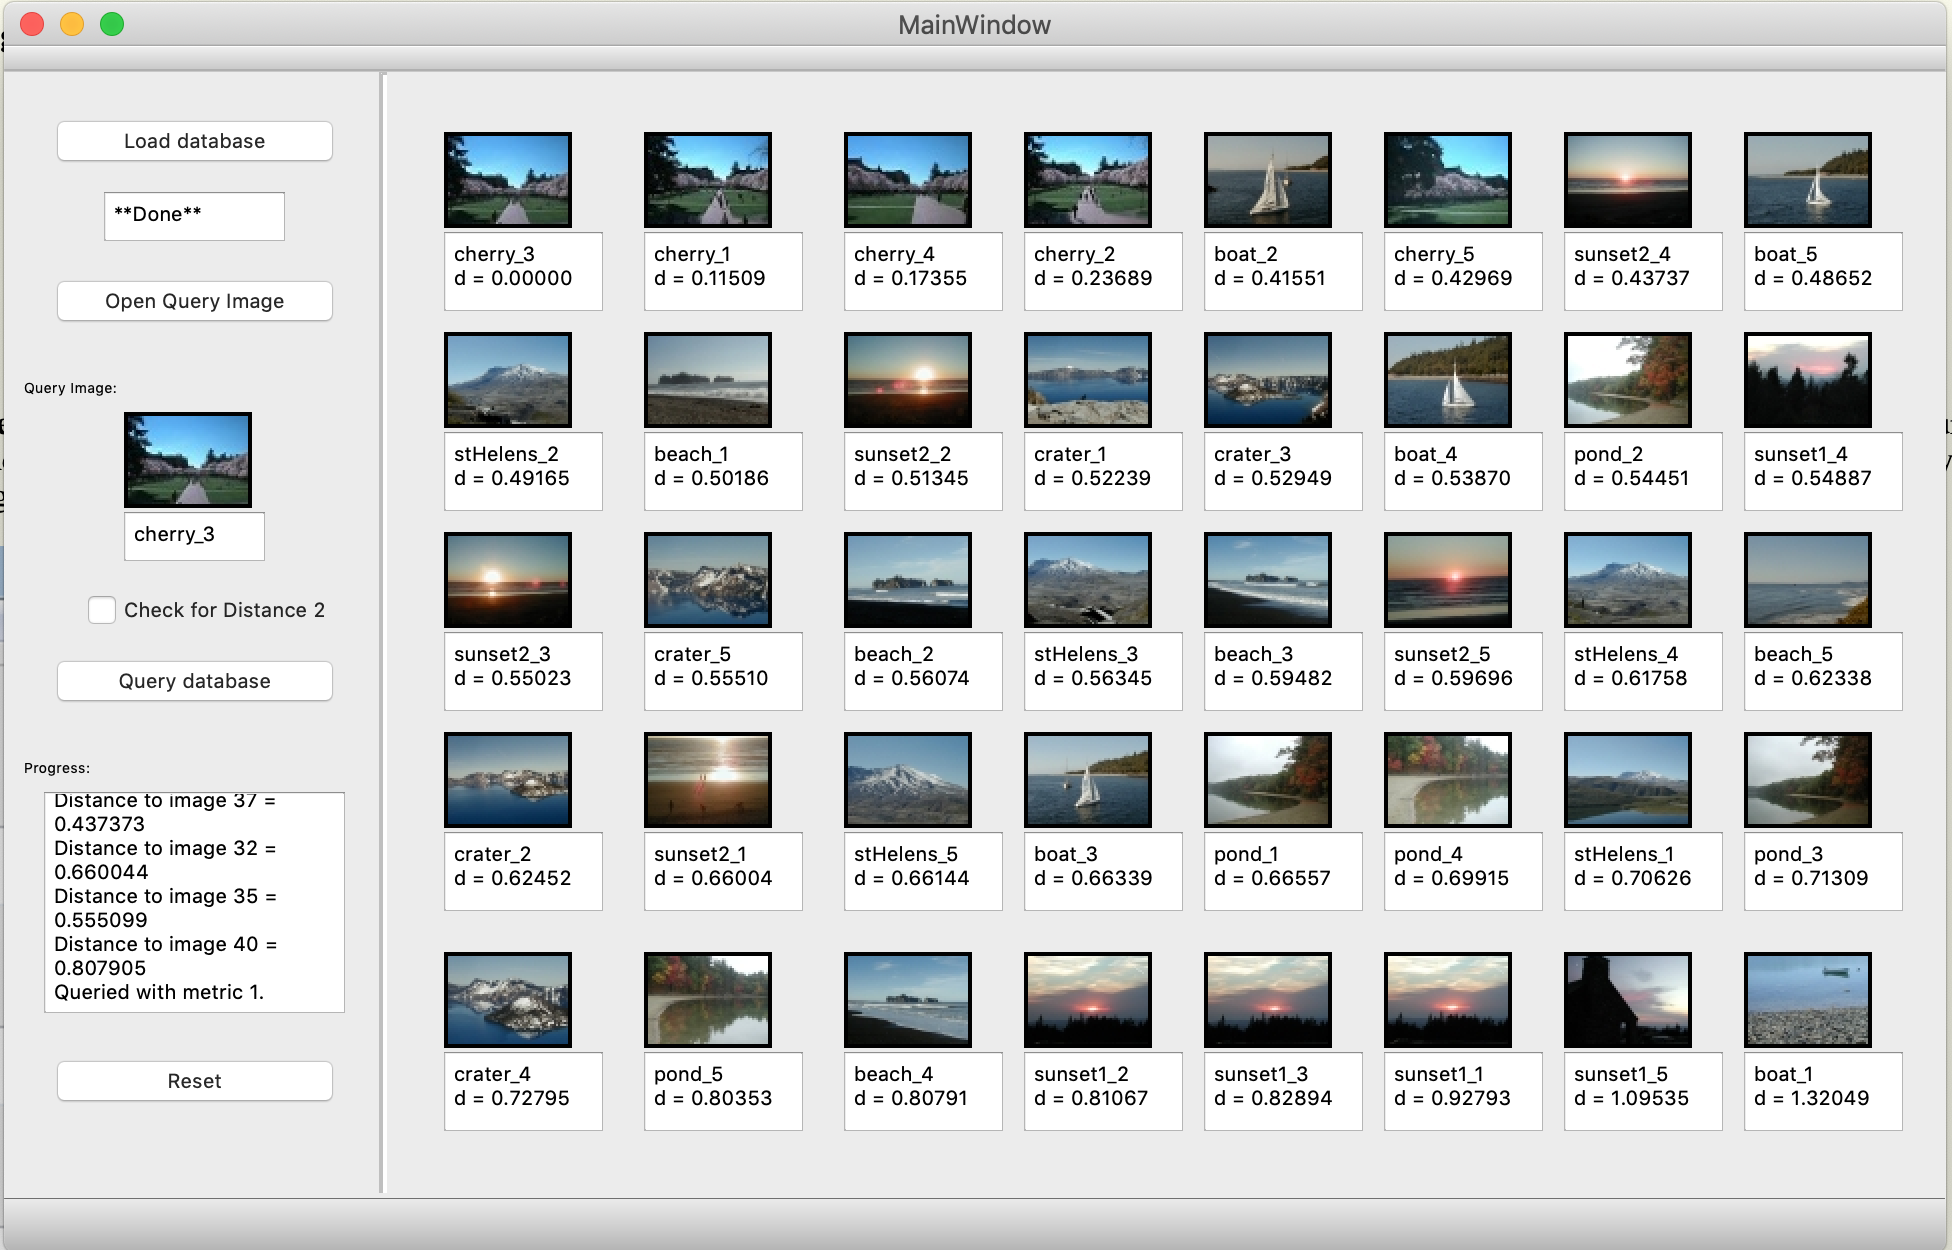
\includegraphics[width=\textwidth]{cherry_3_distance1.png}
  
  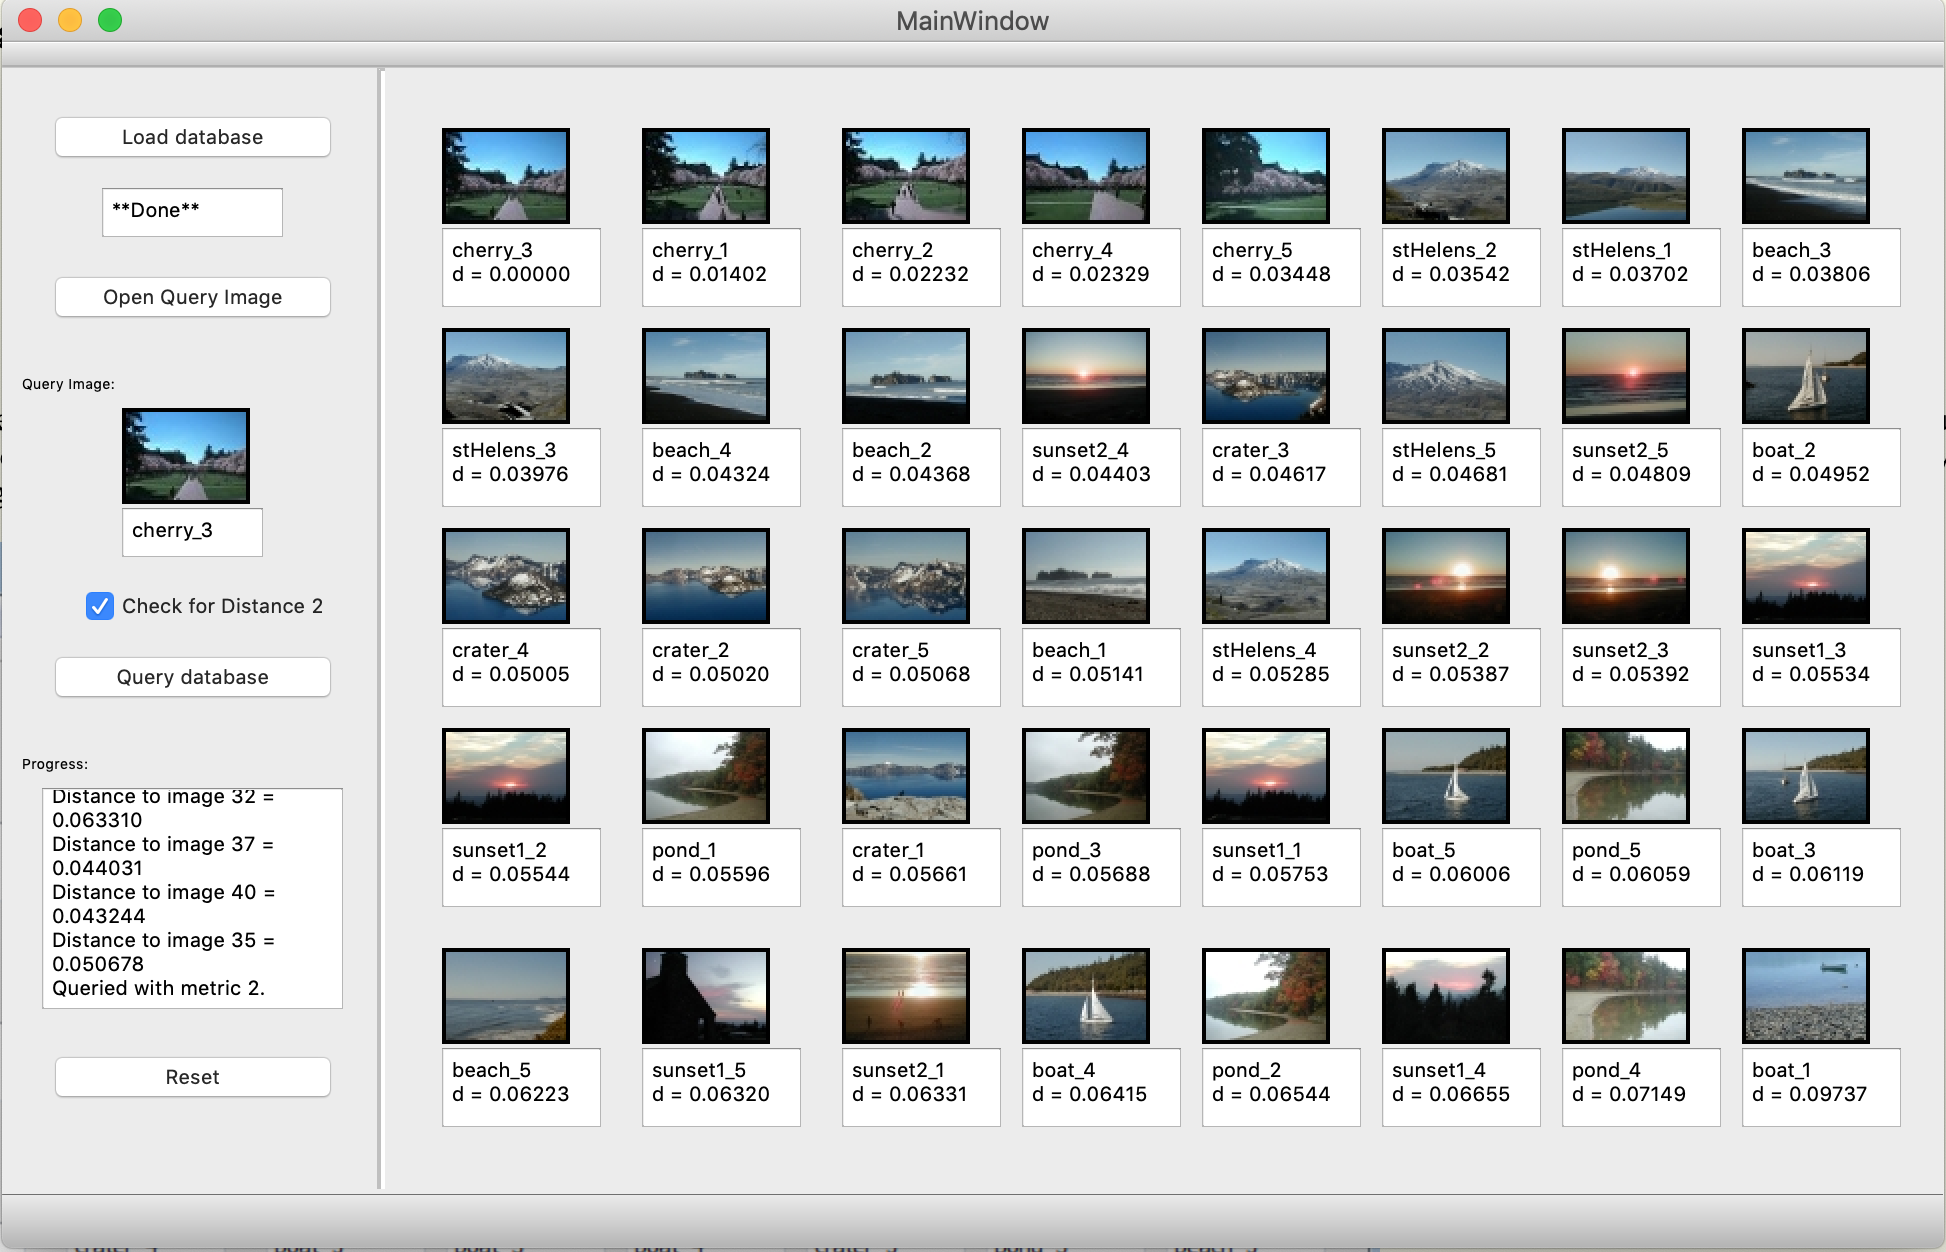
\includegraphics[width=\textwidth]{cherry_3_distance2.png}
  
  Query results for \texttt{cherry\_3.jpg}.
\end{center}

These queries were among the easiest. $d_1$ is near-perfect barely missing
$\texttt{cherry\_5}$, while $d_2$ retrieves all the relevant images as its top results.

\subsection{\texttt{crater}}

\begin{center}
  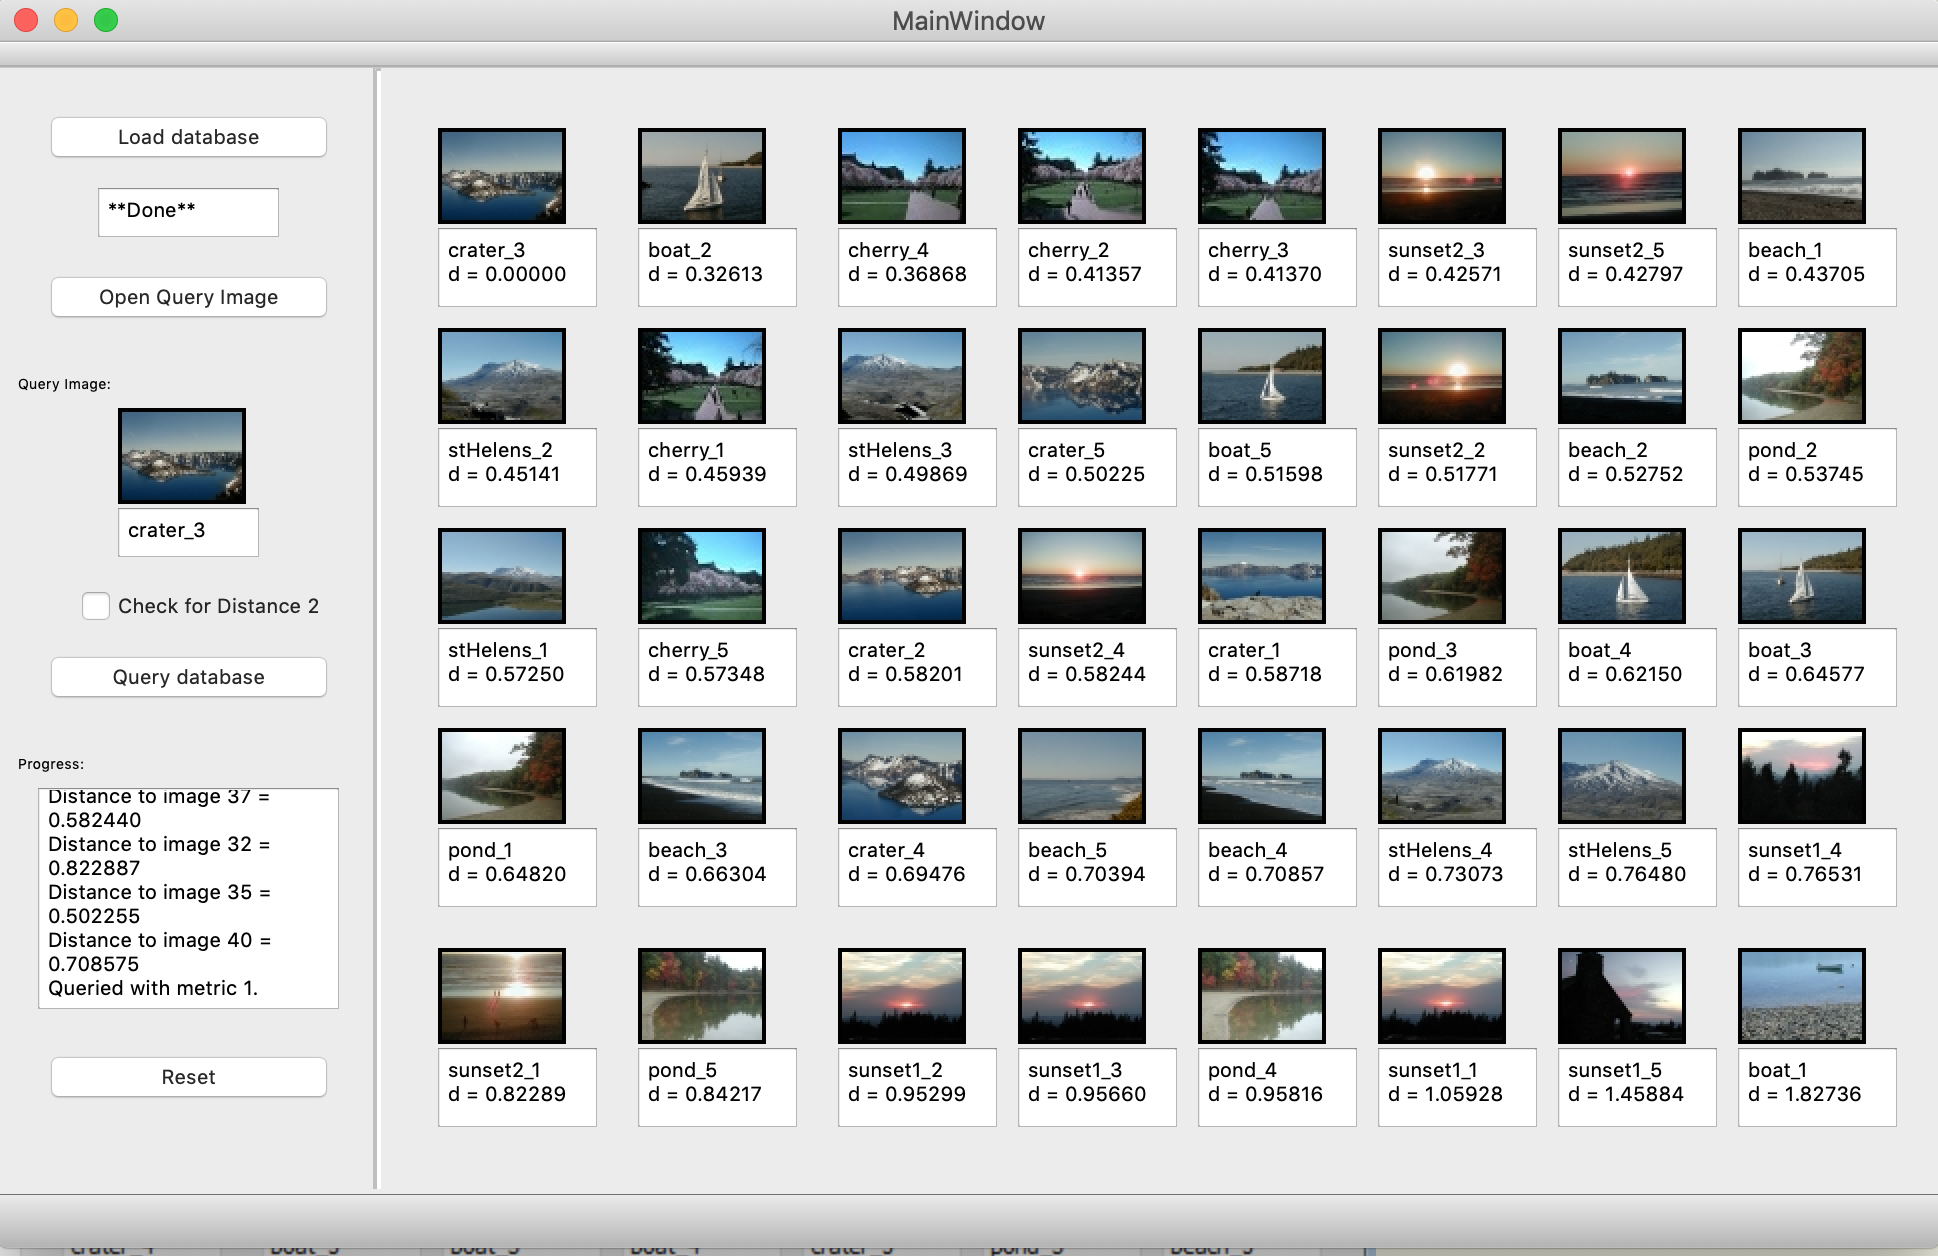
\includegraphics[width=\textwidth]{crater_3_distance1.png}
  
  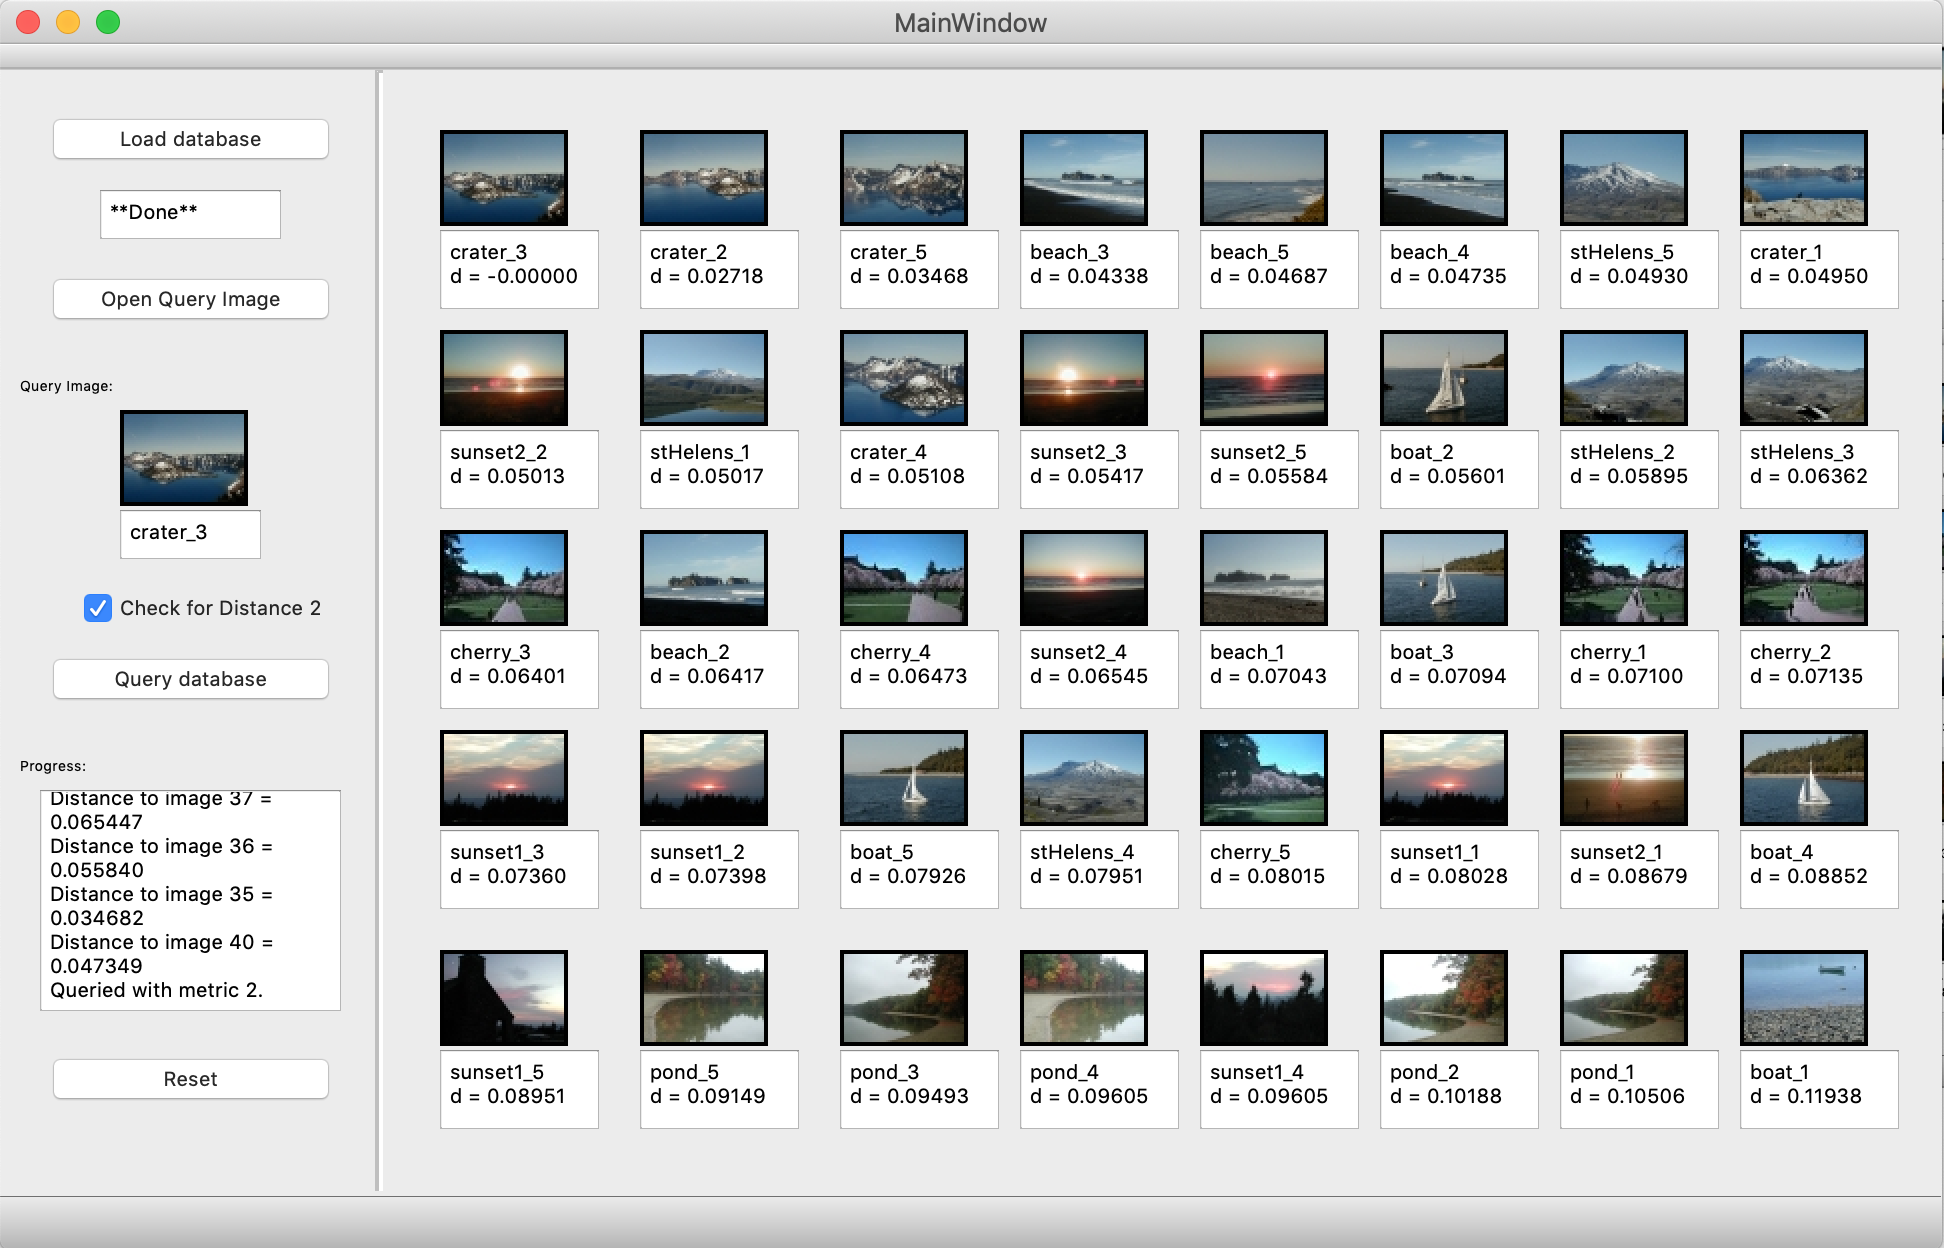
\includegraphics[width=\textwidth]{crater_3_distance2.png}
  
  Query results for \texttt{crater\_3.jpg}.  
\end{center}

$d_1$ completely fails here and doesn't return any relevant images in the top
row. $d_2$ does respectably retrieving $2/4$ crater images with an additional
crater image in the top row.

\subsection{\texttt{pond}}

\begin{center}
  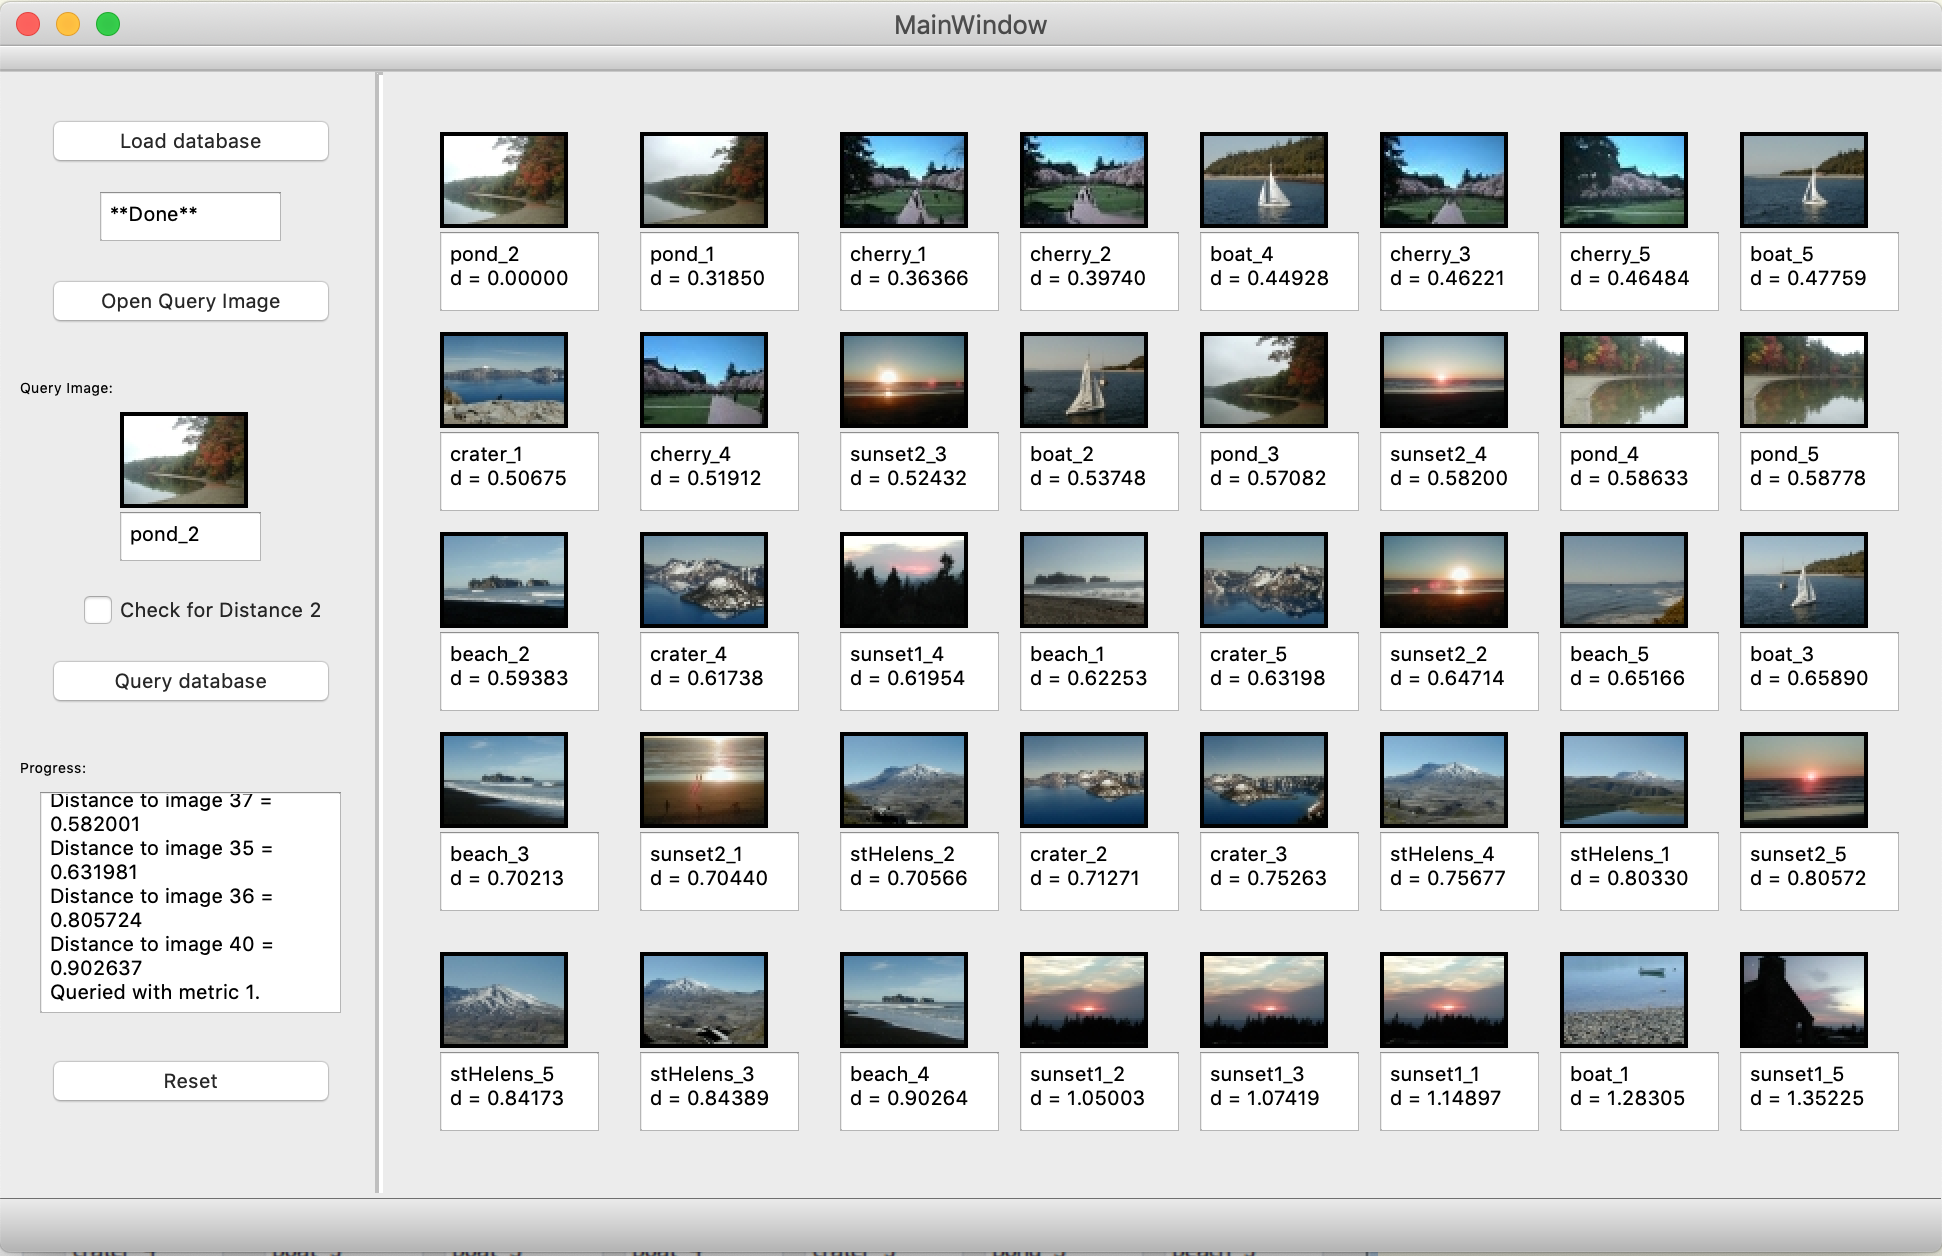
\includegraphics[width=\textwidth]{pond_2_distance1.png}
  
  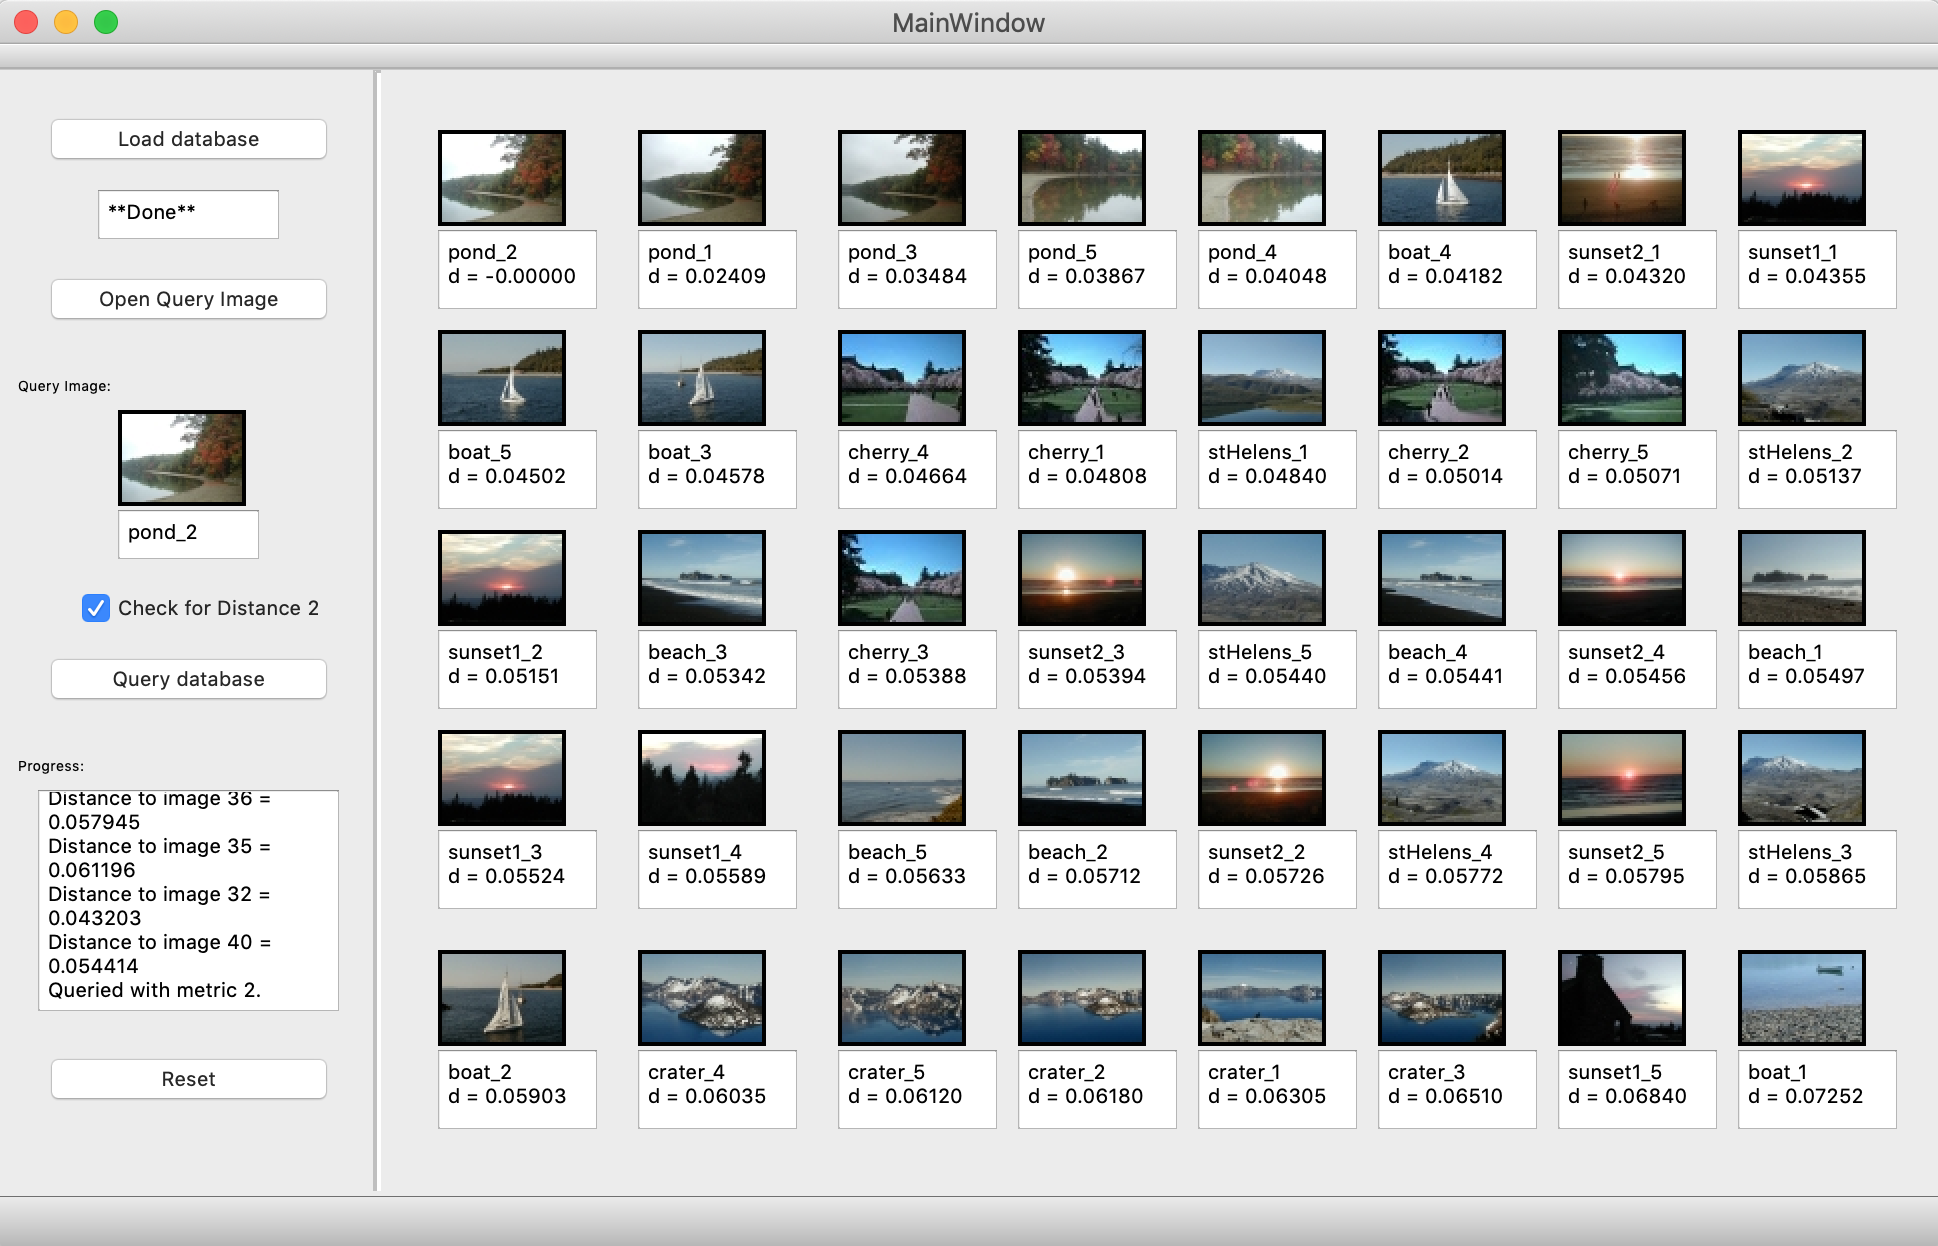
\includegraphics[width=\textwidth]{pond_2_distance2.png}
  
  Query results for \texttt{pond\_2.jpg}.  
\end{center}

$d_1$ mostly fails here. While its top result is another pond image, the other 3
are nowhere to be found in the top row. $d_2$ does perfectly: its top 4 results
are the other 4 pond images.

\subsection{\texttt{stHelens}}

\begin{center}
  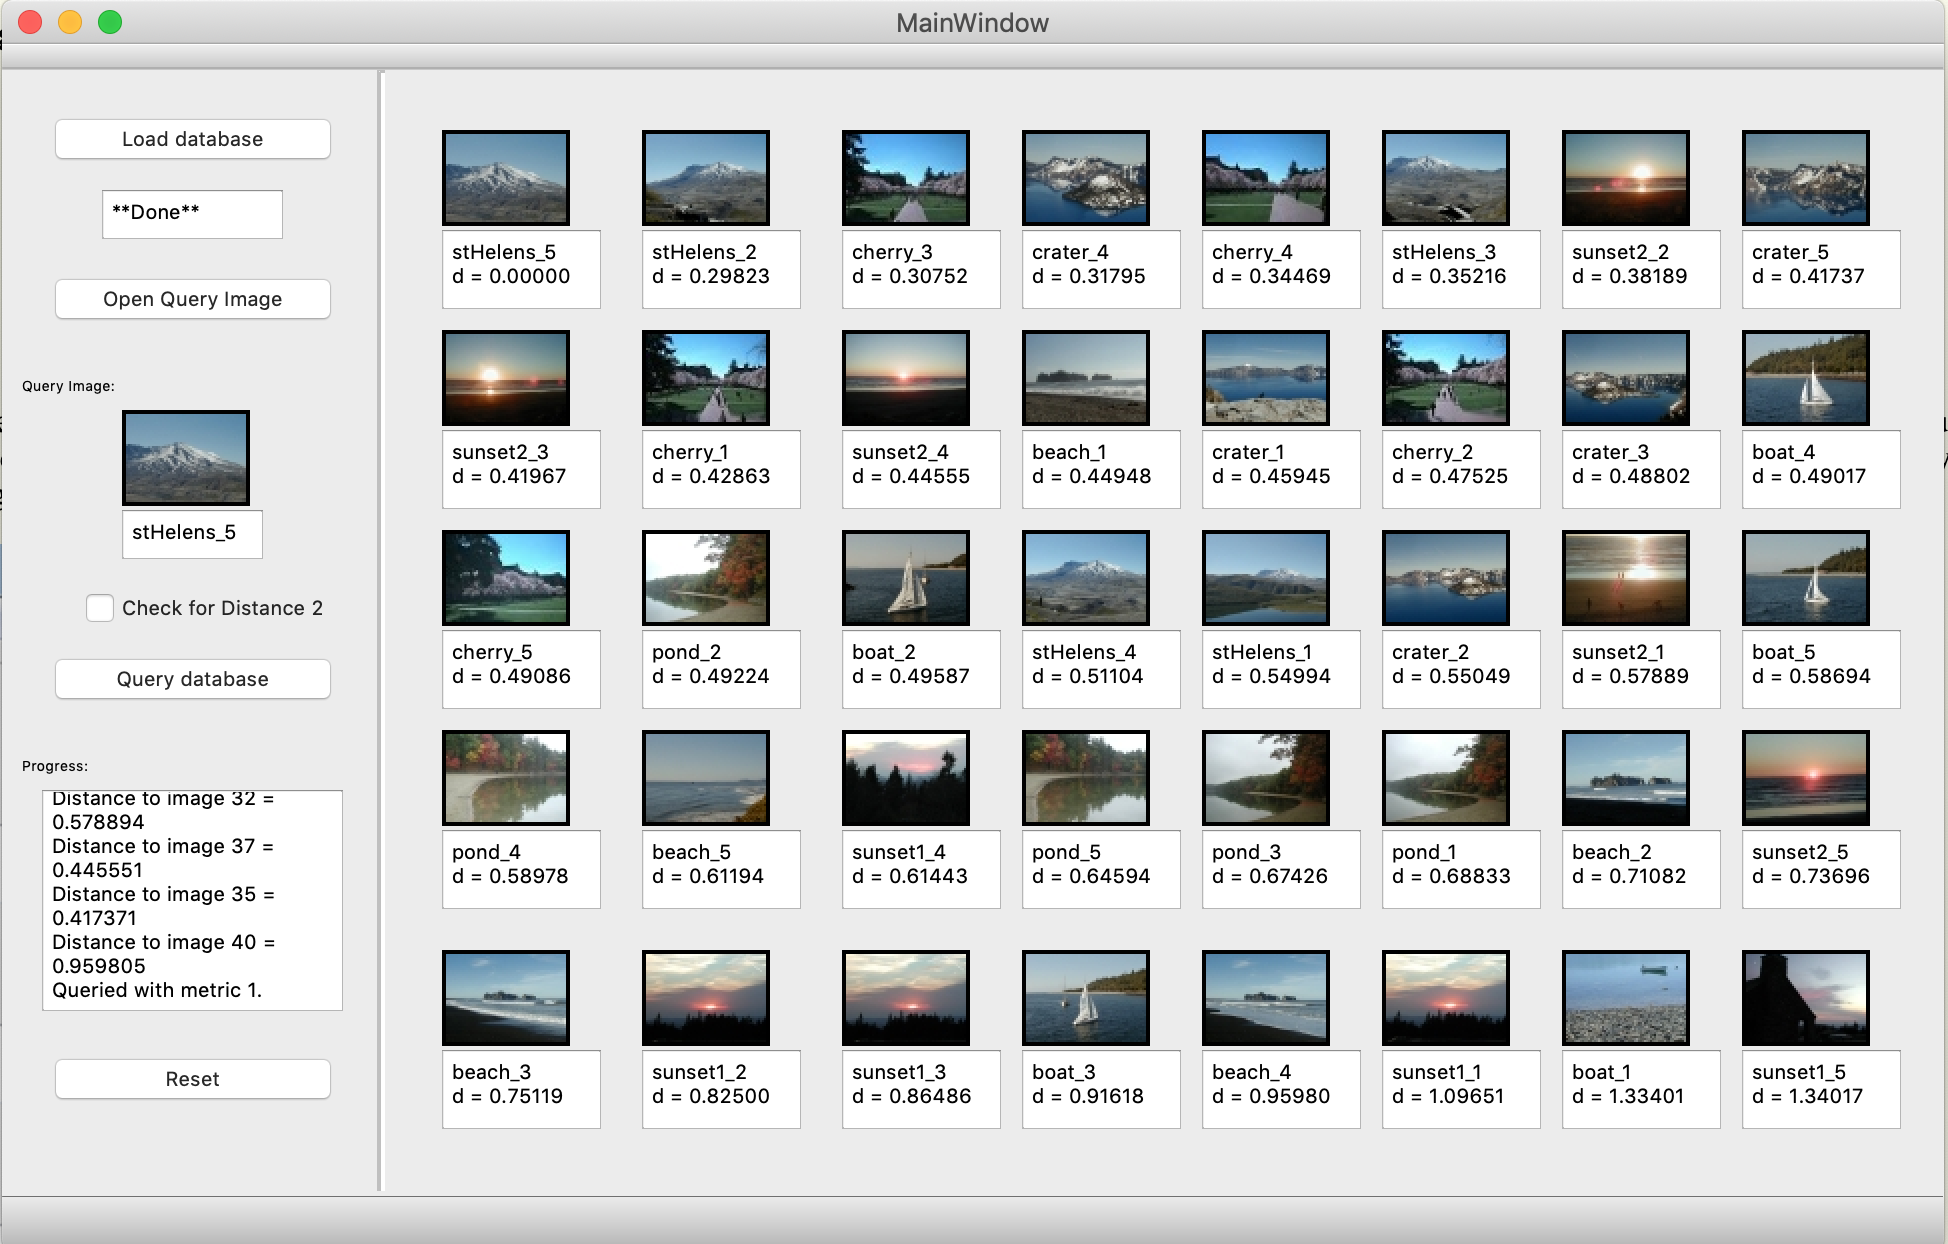
\includegraphics[width=\textwidth]{stHelens_5_distance1.png}
  
  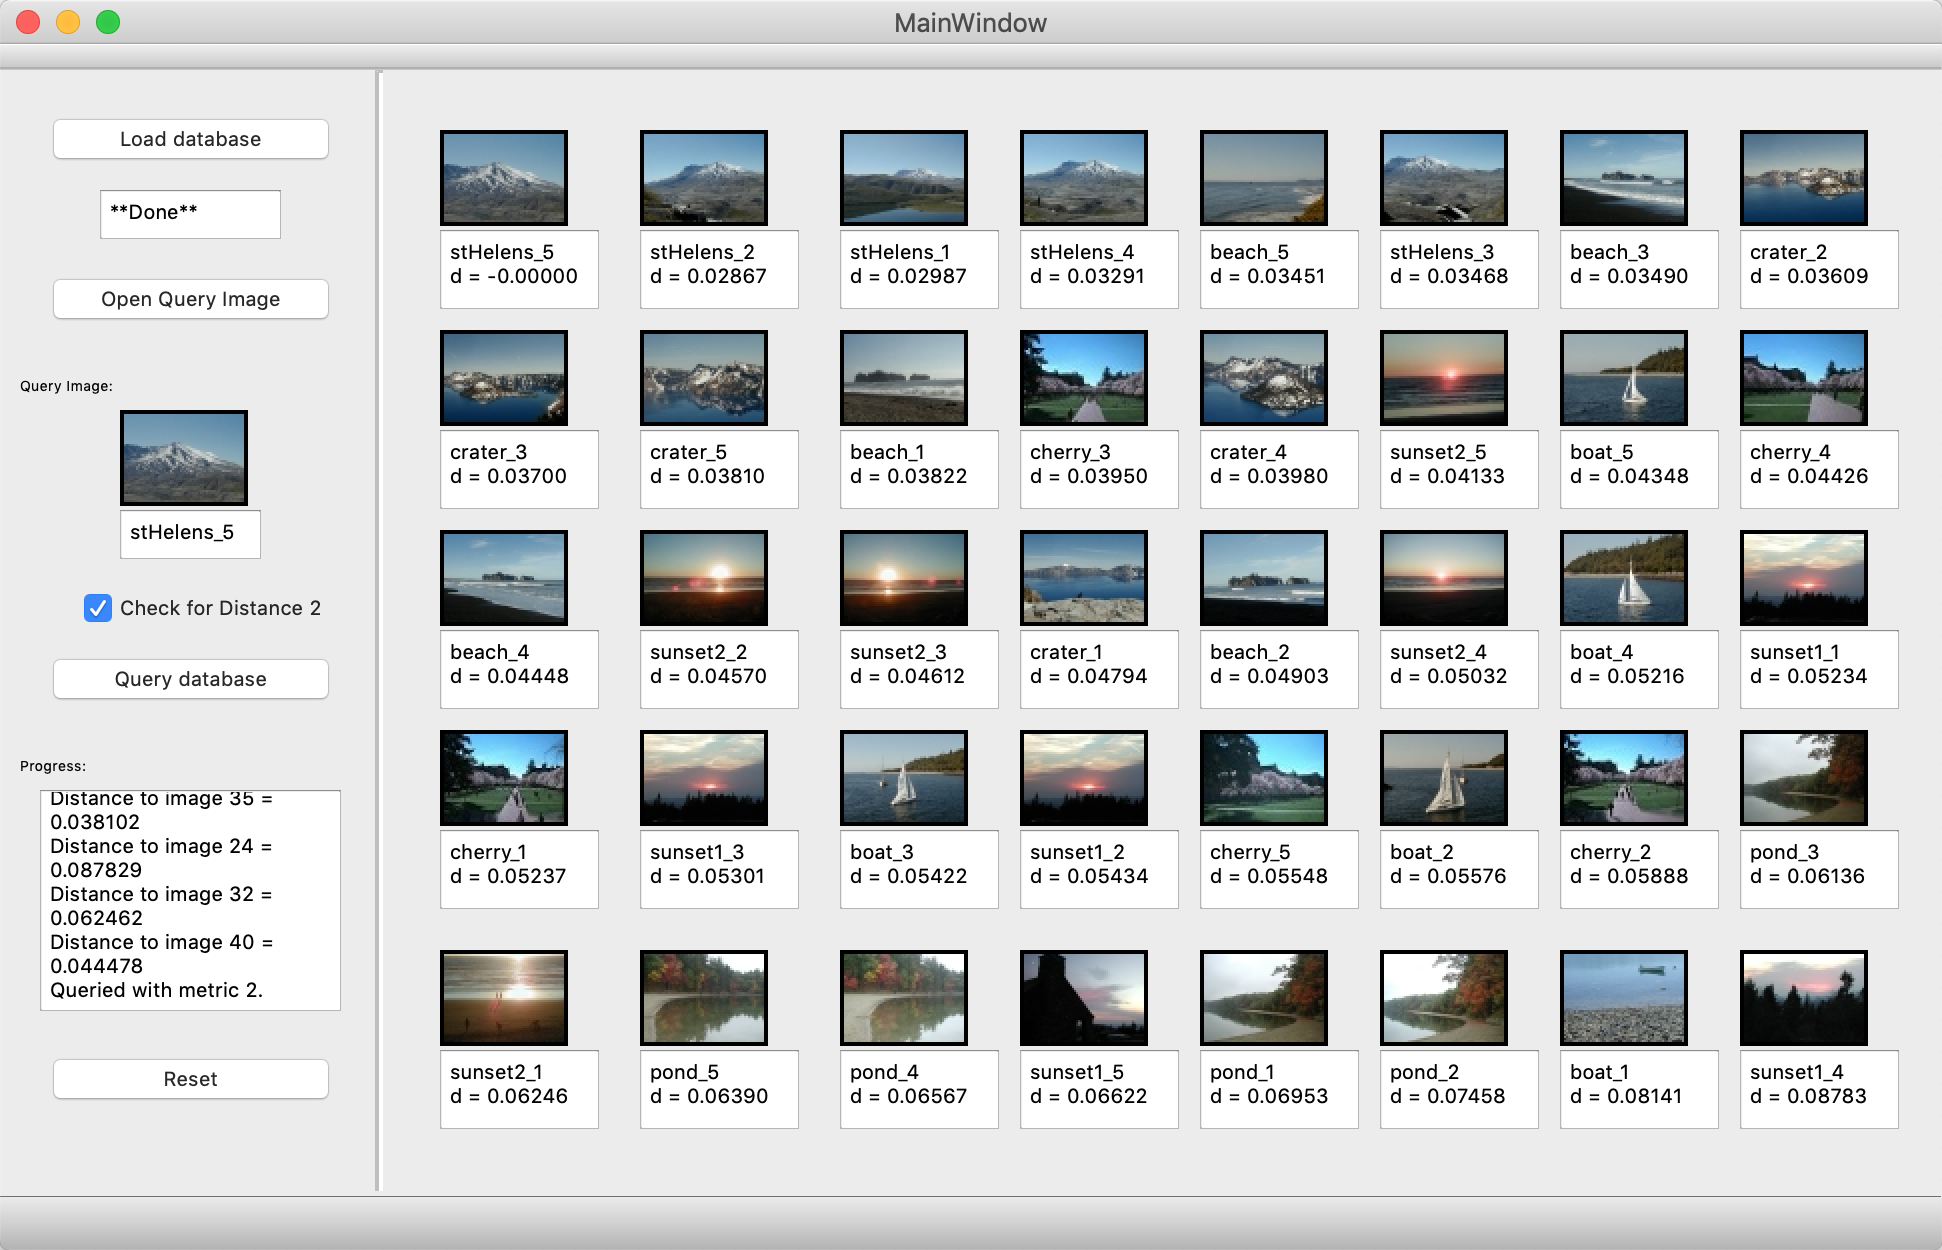
\includegraphics[width=\textwidth]{stHelens_5_distance2.png}
  
  Query results for \texttt{stHelens\_5.jpg}.  
\end{center}

$d_1$ does okay returning another image of Mount St. Helens as its top result
with another in the top row. $d_2$ does very well with its top 3
results being of Mount St. Helens and narrowly missing \texttt{stHelens\_3}.

\subsection{\texttt{sunset1}}

\begin{center}
  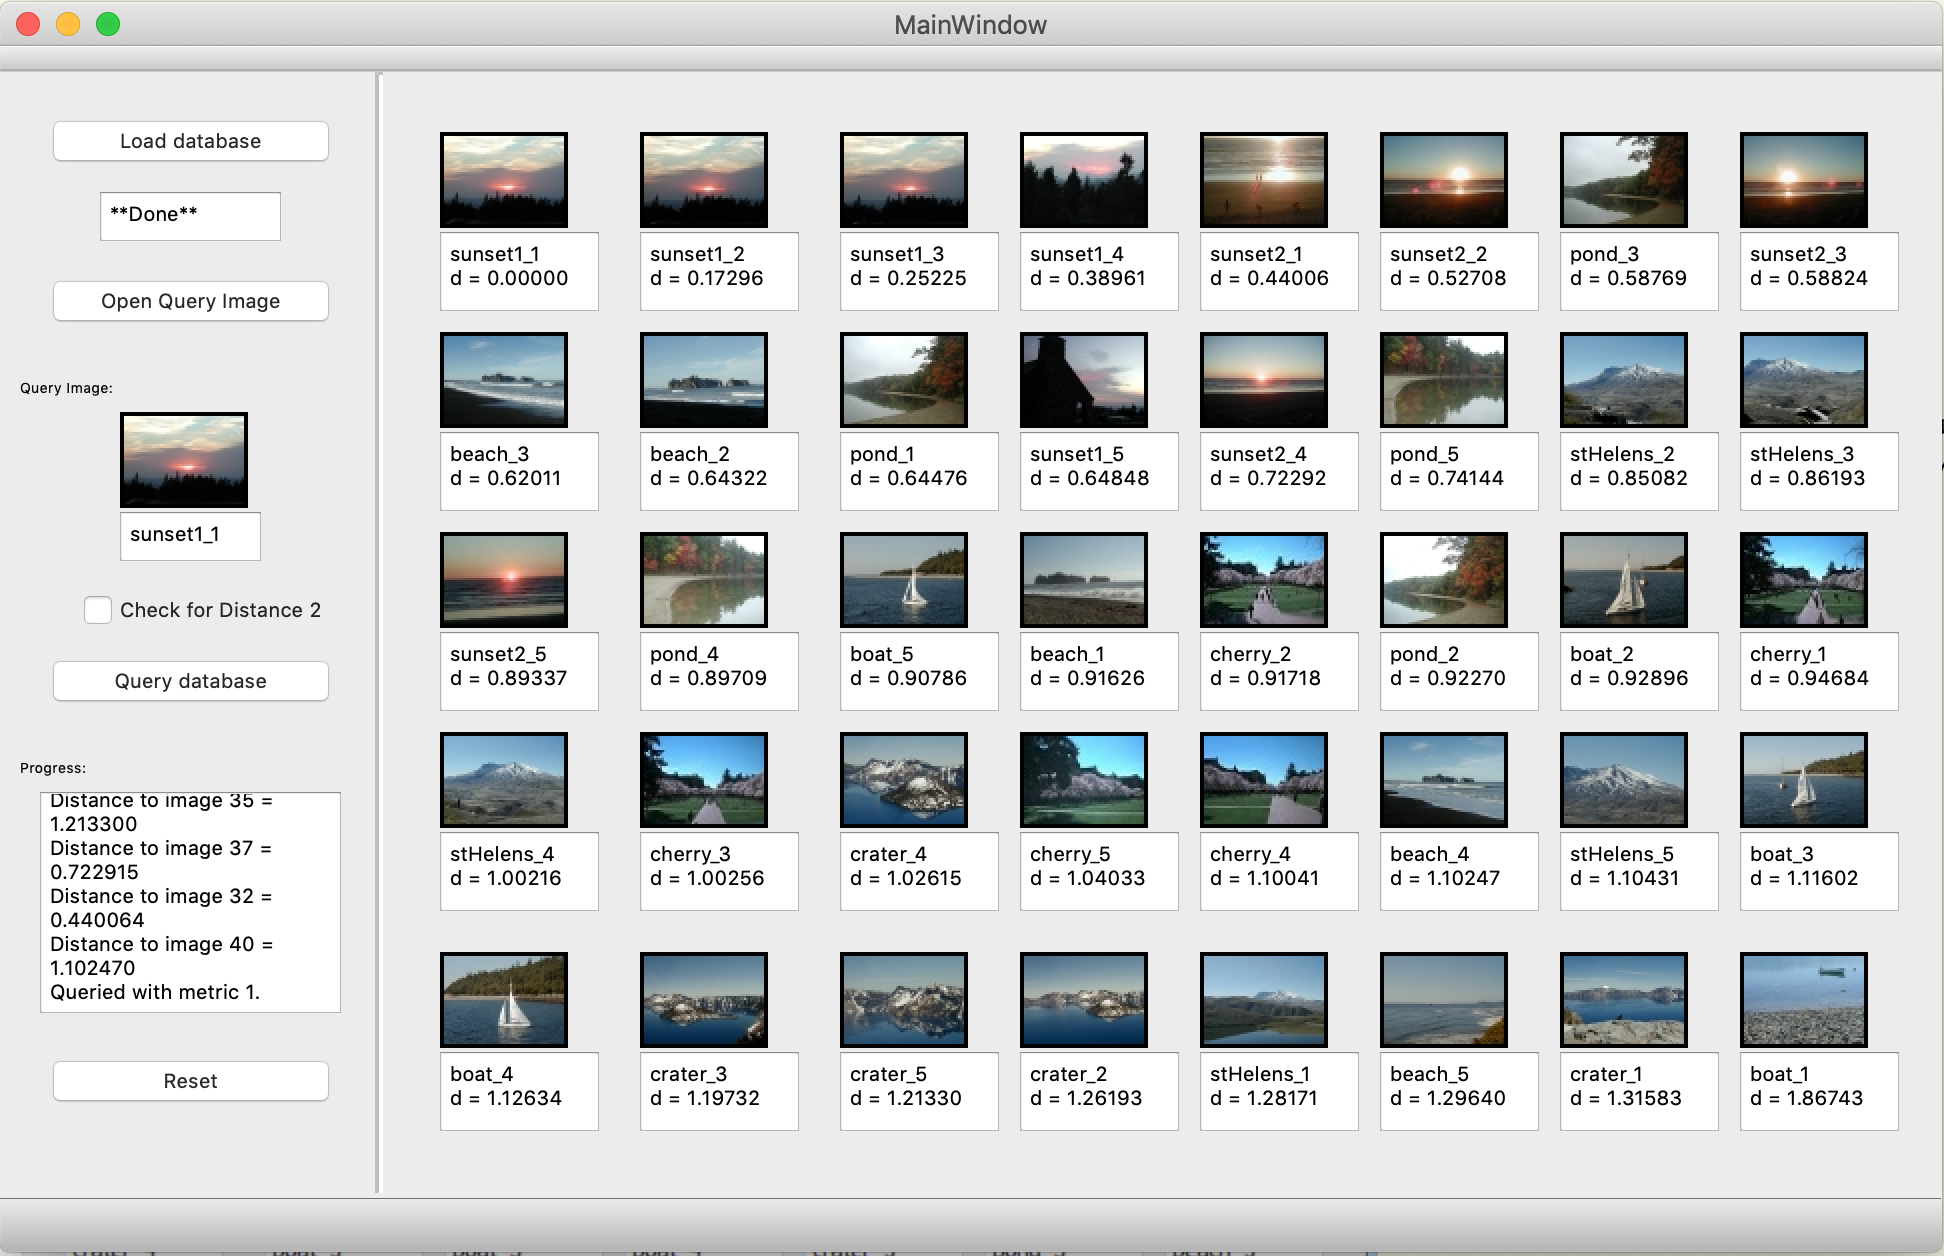
\includegraphics[width=\textwidth]{sunset1_1_distance1.png}
  
  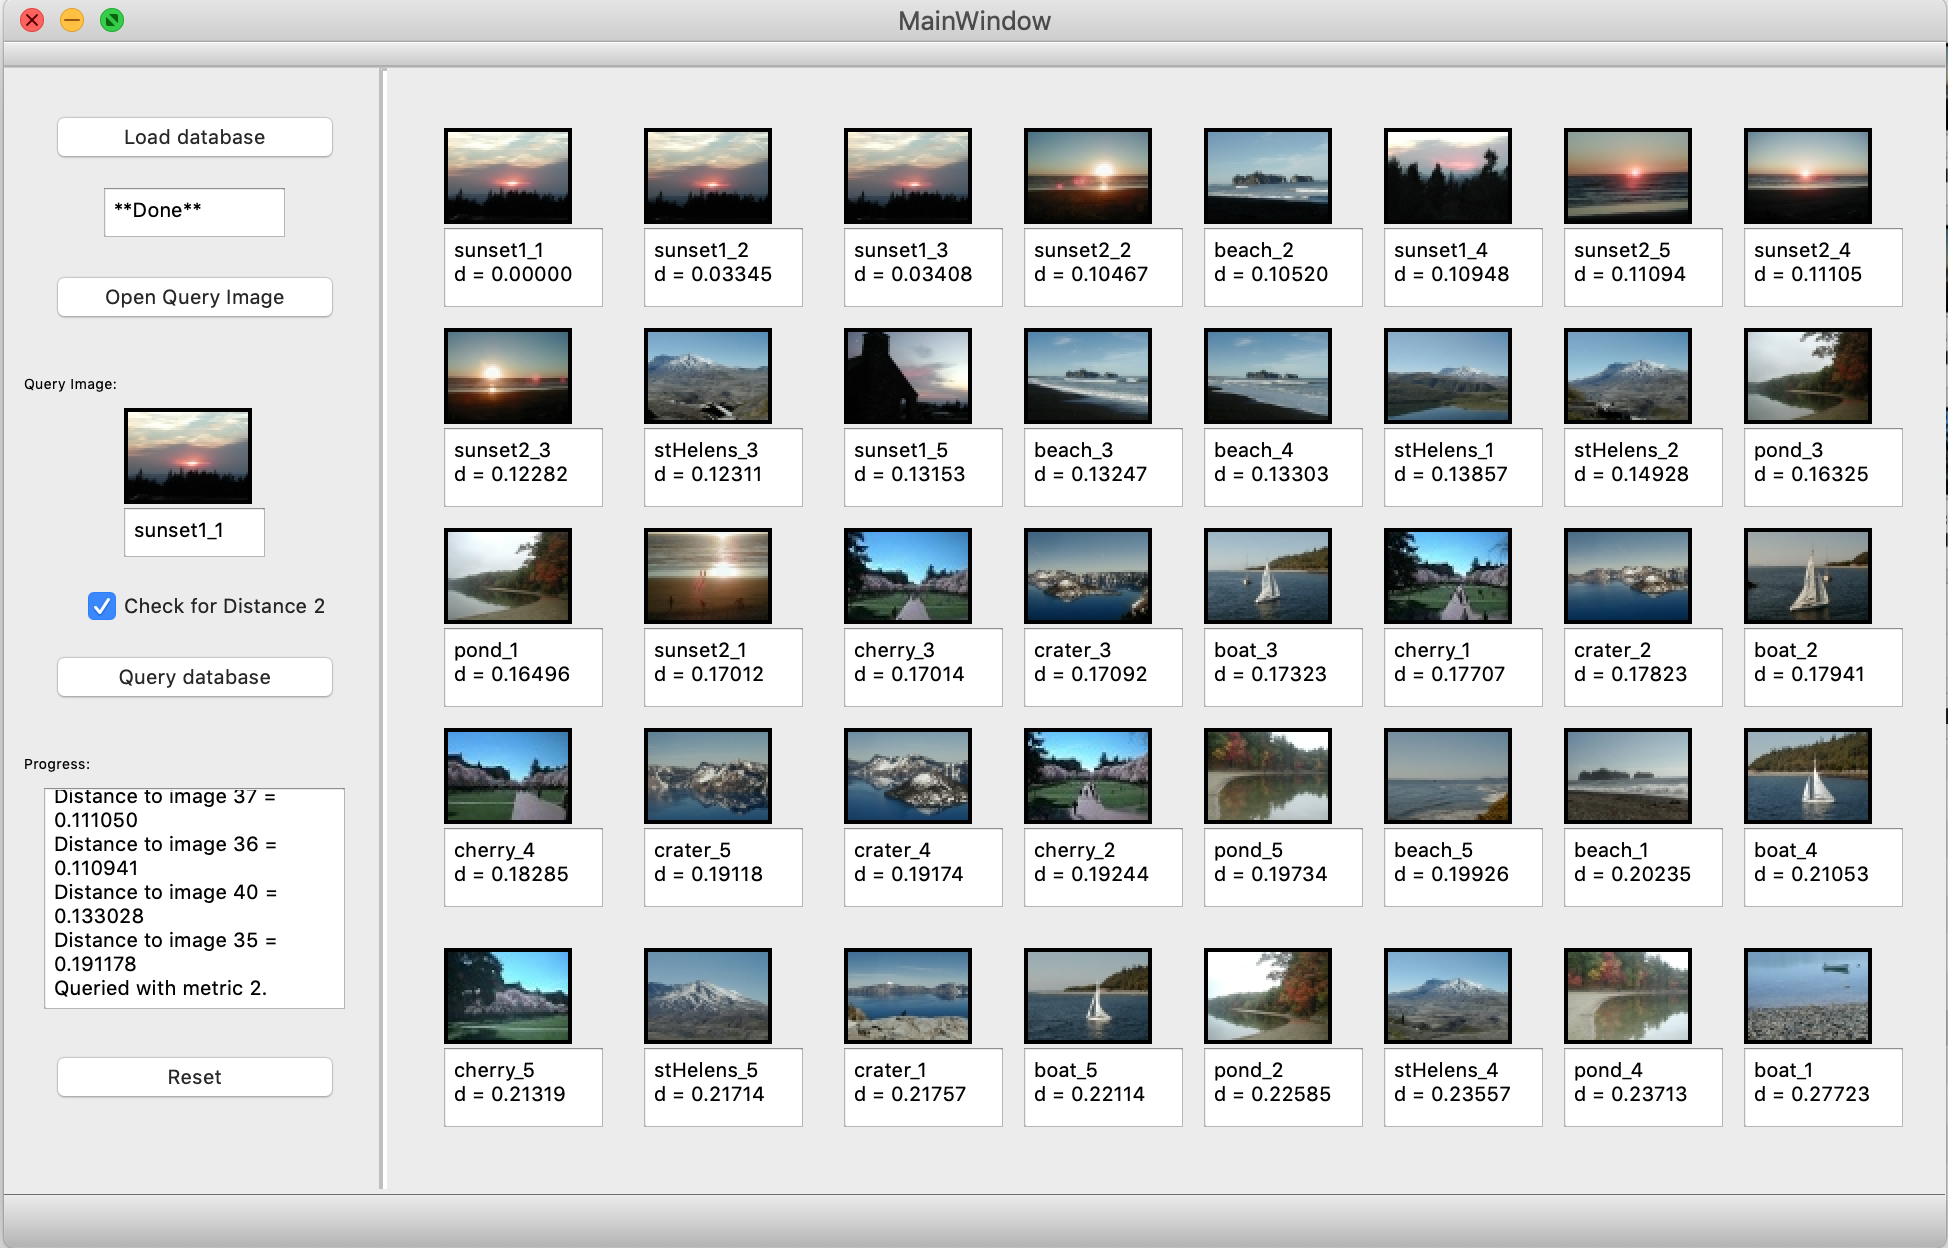
\includegraphics[width=\textwidth]{sunset1_1_distance2.png}
  
  Query results for \texttt{sunset1\_1.jpg}.  
\end{center}

Both $d_1$ and $d_2$ seem to do equally well here. The top row is all sunsets
except for one image in both cases.

\subsection{\texttt{sunset2}}

\begin{center}
  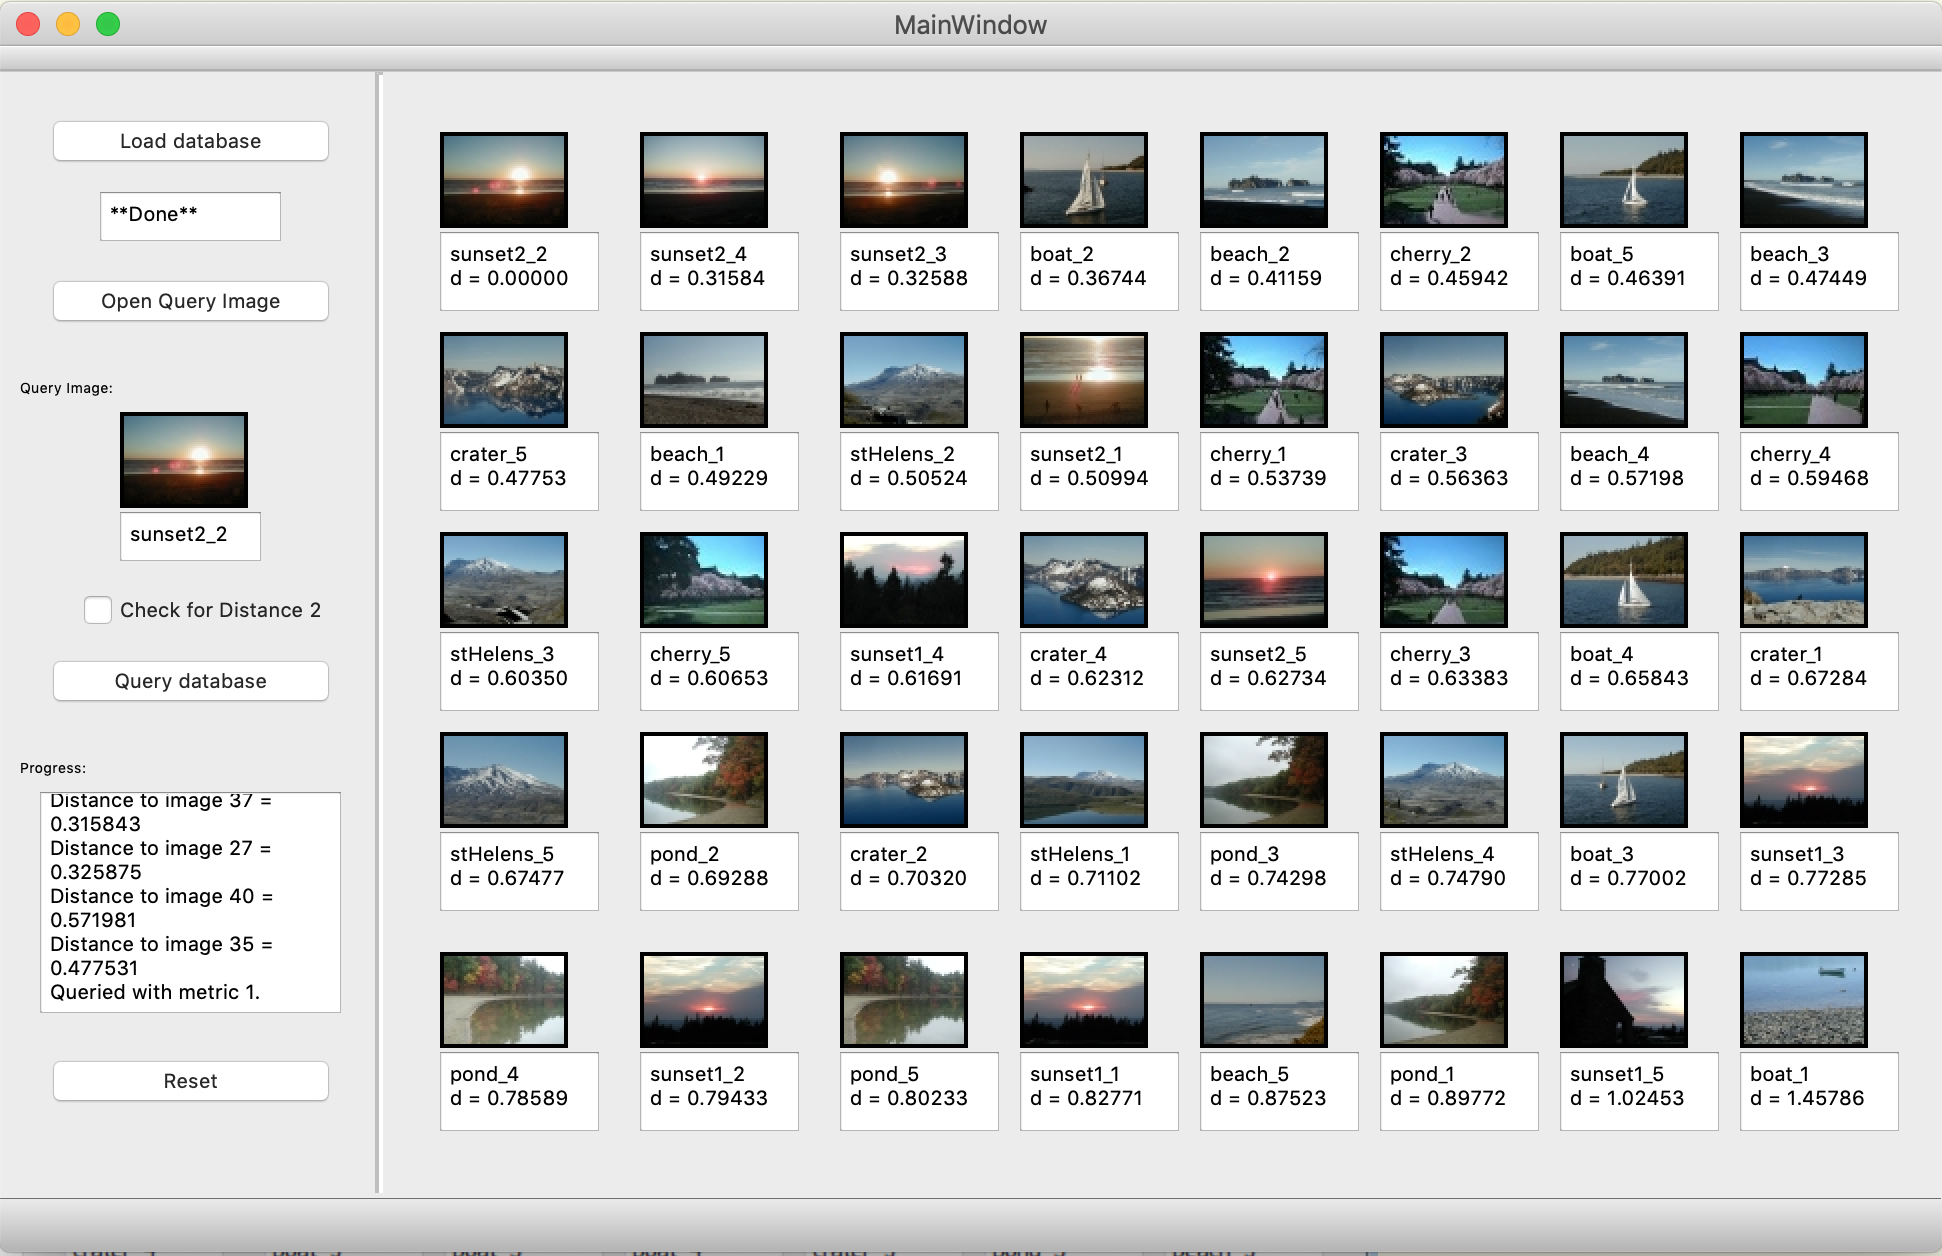
\includegraphics[width=\textwidth]{sunset2_2_distance1.png}
  
  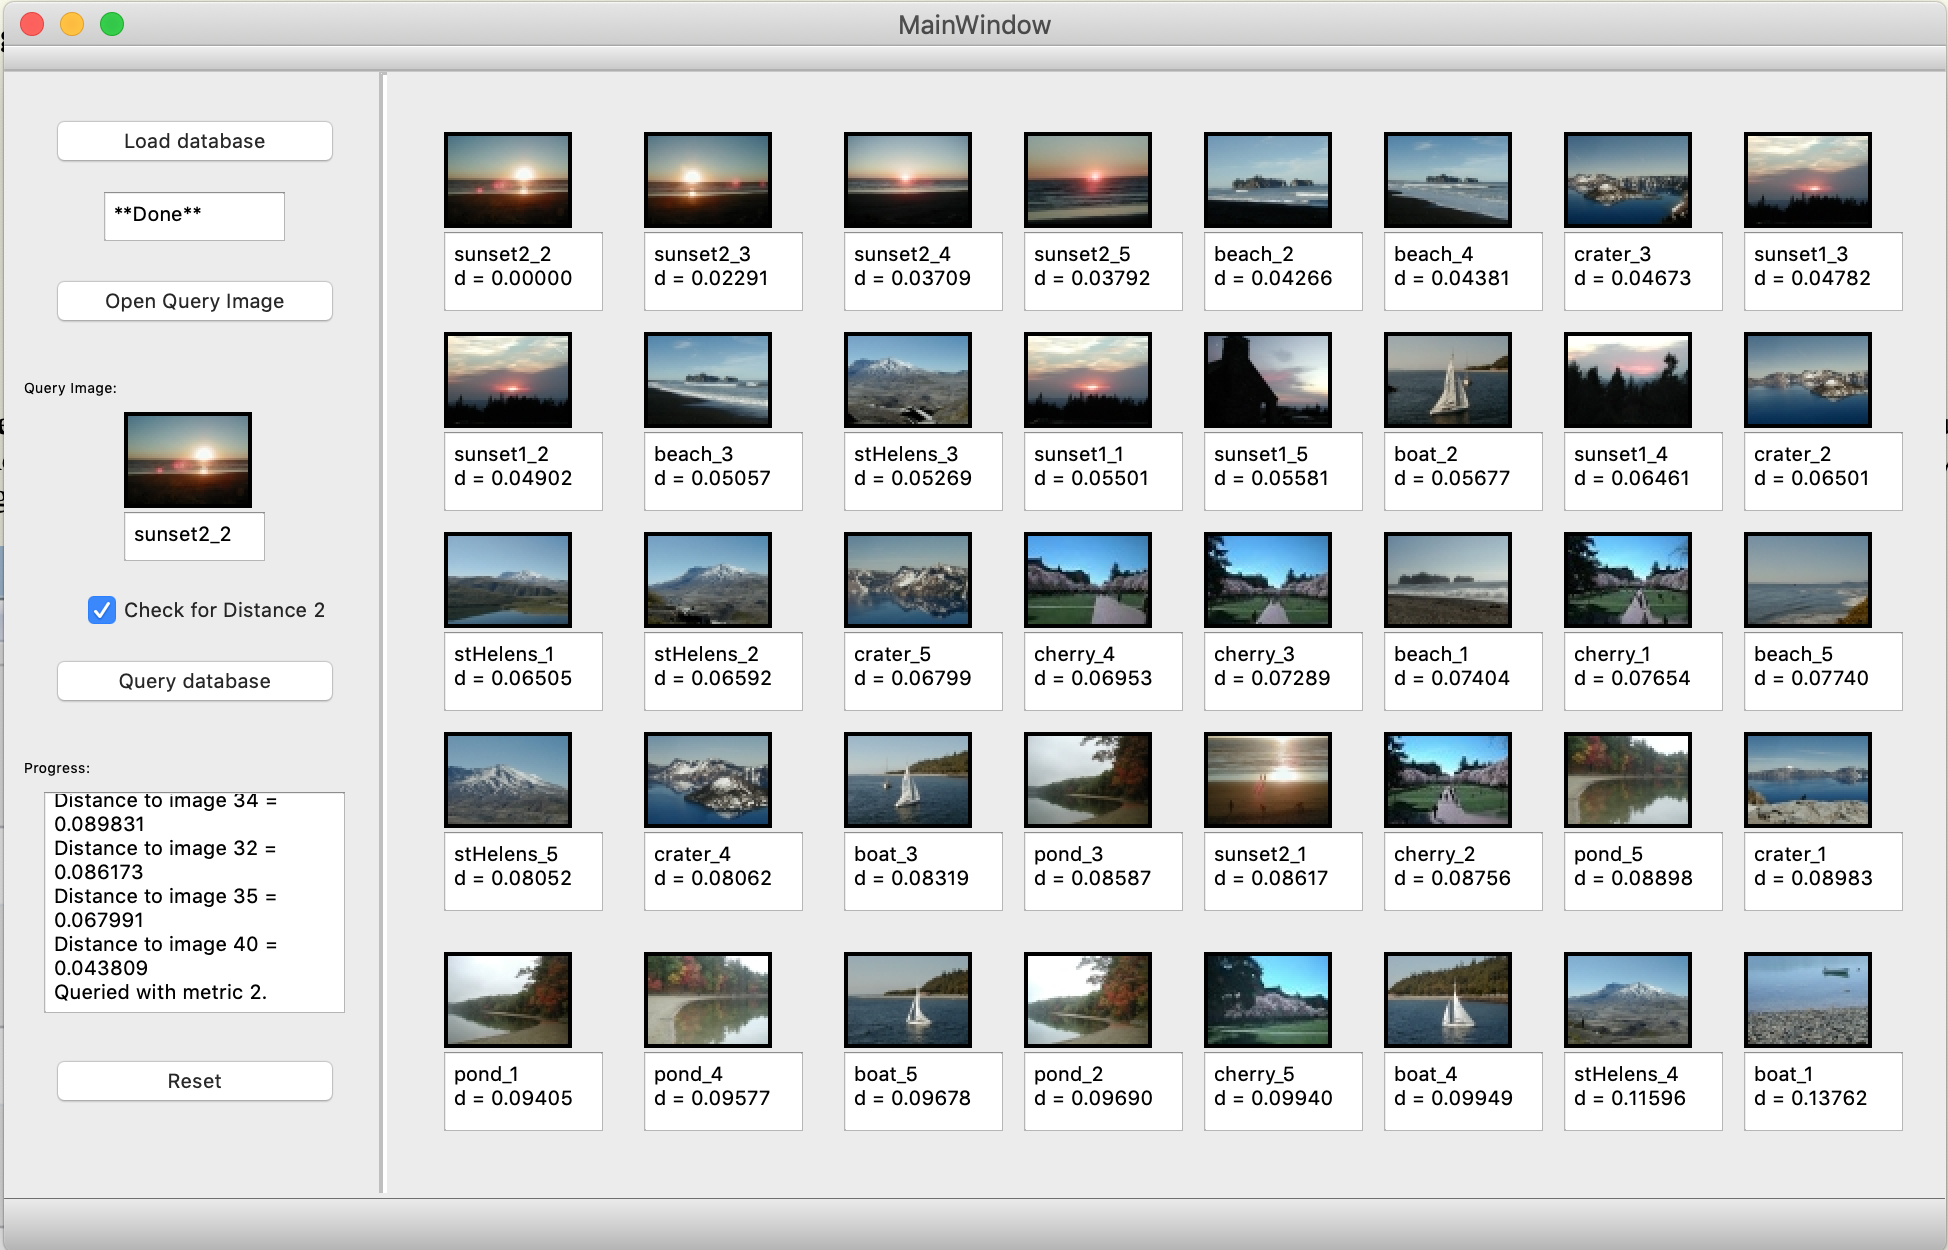
\includegraphics[width=\textwidth]{sunset2_2_distance2.png}
  
  Query results for \texttt{sunset2\_2.jpg}.  
\end{center}

This sunset is more challenging. $d_1$'s top two results are sunsets, but $d_2$
does better: its top 3 results are sunsets with an additional result in the top
row.

\section*{Appendix}

All code used to generate these images can be found at
\href{https://github.com/ppham27/cse576/blob/master/hw3}{\texttt{ppham27/cse576/hw3}}. The
embedded JPEG, PNG files, and the \LaTeX can be found in
\href{https://github.com/ppham27/cse576/blob/master/hw3/report}{\texttt{ppham27/cse576/hw3/report}}.

\end{document}
